% Task C15
% Source volume: lower
% Physical scan pages: 91--117
% Printed book pages: 79--105
% Transcribe only source content; omit running headers, footers, and printed page numbers.
\chapter{Fourier 级数}

Fourier 级数是幂级数之外的另一类重要的函数项级数，它的出现对于现代数学的理论发展和实际应用都有重大意义。本章只讨论 Fourier 级数理论的一些基础知识。§15.1 为有关 Fourier 系数的各种性质，§15.2 讨论 Fourier 级数在各种意义下的收敛性问题。最后一节为学习要点和参考题。

\section{Fourier 系数}

Fourier 级数是一类特殊的三角级数，它的特殊性在于其系数是从某个可积函数出发经过 Euler-Fourier 公式计算出来的。

\subsection{Fourier 系数的计算公式}

设 $f$ 是以 $2\pi$ 为周期的函数且在 $[-\pi,\pi]$ 上可积和绝对可积。（若 $f$ 为常义可积，则可积蕴含绝对可积，又若 $f$ 为广义可积，则绝对可积蕴含可积。）

计算 $f$ 的 Fourier 系数的 Euler-Fourier 公式是：
\begin{equation}
  a_n=\frac1\pi\int_{-\pi}^{\pi}f(x)\cos nx\,\dd x,\quad n=0,1,2,\ldots;
  \tag{15.1}
  \label{eq:15.1}
\end{equation}
\begin{equation}
  b_n=\frac1\pi\int_{-\pi}^{\pi}f(x)\sin nx\,\dd x,\quad n=1,2,\ldots.
  \tag{15.2}
  \label{eq:15.2}
\end{equation}
如果三角级数
\[
  \frac{a_0}{2}+\sum_{n=1}^{\infty}(a_n\cos nx+b_n\sin nx)
\]
中的系数满足公式 (15.1) 和 (15.2)，则称该三角级数是 $f$ 的 Fourier 级数，记为
\begin{equation}
  f(x)\sim\frac{a_0}{2}+\sum_{n=1}^{\infty}(a_n\cos nx+b_n\sin nx).
  \tag{15.3}
  \label{eq:15.3}
\end{equation}

\begin{xremark}
上述公式只表明右边的系数 $a_n,b_n$ 与左边的函数 $f$ 之间满足公式 (15.1) 和 (15.2)。记号“$\sim$”没有其他含义，公式 (15.3) 右边的级数是否收敛，以及在收敛时其和函数是否等于 $f$，都是需要另行讨论的问题。
\end{xremark}

回顾教科书中导出 Euler-Fourier 公式的过程，其出发点是在 $(-\infty,+\infty)$ 上一致收敛（也就是在一个周期长度的闭区间上一致收敛）的一个三角级数，然后通过逐项求和导出上述公式。由此就得到 Fourier 级数学习中的第一个基本定理（其中对一致收敛的范围理解如上）：

\begin{xproposition}[15.1.1]
一致收敛的三角级数必是其和函数的 Fourier 级数。
\end{xproposition}

虽然用 Euler-Fourier 公式得到的 Fourier 级数未必一致收敛，但这个命题仍然是很有用的一个基本结果。

\begin{xremark}
虽然只有周期函数才可能有 Fourier 级数，但当 $f$ 的定义域是某个长度为 $2\pi$ 的区间时，可先将其延拓成周期函数，且把延拓后的周期函数的 Fourier 级数称为 $f$ 在该区间上的 Fourier 级数。对于周期不是 $2\pi$ 的周期函数或只在长度不是 $2\pi$ 的区间上定义的函数，也可用类似的方法定义它们的 Fourier 级数。
\end{xremark}

\begin{xremark}
当 $f$ 为偶函数或奇函数时，$f$ 的 Fourier 级数有较为简单的形式：当 $f$ 为偶函数时，所有的 $b_n$ 均为 0，并且 (15.1) 成为
\begin{equation}
  a_n=\frac2\pi\int_0^{\pi}f(x)\cos nx\,\dd x,\quad n=0,1,2,\ldots;
  \tag{15.4}
  \label{eq:15.4}
\end{equation}
当 $f$ 为奇函数时，所有的 $a_n$ 均为 0，并且 (15.2) 成为
\begin{equation}
  b_n=\frac2\pi\int_0^{\pi}f(x)\sin nx\,\dd x,\quad n=1,2,\ldots.
  \tag{15.5}
  \label{eq:15.5}
\end{equation}
这时 $f$ 的 Fourier 级数中只出现含有余弦函数的项与常数项或只出现含有正弦函数的项，分别称为余弦级数或正弦级数。
\end{xremark}

\begin{xremark}
从公式 (15.4) 不难看出，如果 $f$ 在 $[0,\pi]$ 上具有某种对称性，例如关于点 $(\pi/2,0)$ 为偶函数（奇函数），则可以证明在公式 (15.4) 中当 $n$ 为奇数（偶数）时积分为 0。对于公式 (15.5) 有类似的结论（参见上册 10.4.3 小节中的命题和例题）。
\end{xremark}

下一个命题建立 $f$ 的 Fourier 系数与其导函数 $f'$ 的 Fourier 系数之间的联系，这也是 Fourier 系数的基本性质之一：

\begin{xproposition}[15.1.2]
设以 $2\pi$ 为周期的连续函数 $f$ 在 $[-\pi,\pi]$ 上除了有限个点以外可导，又设（在任意补充有限个点上的值之后）$f'$ 在 $[-\pi,\pi]$ 上可积和绝对可积，则从
\[
  f(x)\sim\frac{a_0}{2}+\sum_{n=1}^{\infty}(a_n\cos nx+b_n\sin nx)
\]
就有
\[
  f'(x)\sim\left(\frac{a_0}{2}\right)'+\sum_{n=1}^{\infty}(a_n\cos nx+b_n\sin nx)'
  =\sum_{n=1}^{\infty}(nb_n\cos nx-na_n\sin nx).
\]
若用 $a'_n,b'_n$ 记 $f'$ 的 Fourier 系数，这就等价于
\begin{equation}
  a'_0=0,\quad a'_n=nb_n,\quad b'_n=-na_n,\quad n=1,2,\ldots.
  \tag{15.6}
  \label{eq:15.6}
\end{equation}
\end{xproposition}

\begin{xproof}
因为 $f$ 是以 $2\pi$ 为周期的连续函数，因此 $f(-\pi)=f(\pi)$，由此即可推出 $a'_0=0$。然后由分部积分公式\footnote{这里需要将上册 319 页的分部积分公式 (10.11) 稍作推广，并参见上册 315 页注 2。}可得
\[
  \pi a'_n=\int_{-\pi}^{\pi}f'(x)\cos nx\,\dd x
  =\left.f(x)\cos nx\right|_{-\pi}^{\pi}-\int_{-\pi}^{\pi}f(x)\,\dd(\cos nx)
  =n\int_{-\pi}^{\pi}f(x)\sin nx\,\dd x=n\pi b_n.
\]
这就是 $b_n=a'_n/n$。类似地可以证明 $a_n=-b'_n/n$。
\end{xproof}

\begin{xremark}
对于满足条件的 $f$，公式 (15.6) 可以用于从 $f$ 的 Fourier 系数得到 $f'$ 的 Fourier 系数。这里只需要形式上的“逐项求导”即可。

反之，能否从 $f'$ 的 Fourier 系数得到 $f$ 的 Fourier 系数？从命题的证明可知，如果 $f\in C[-\pi,\pi]$ 但不满足 $f(\pi)=f(-\pi)$，则肯定不行。这时 $a'_0\ne0$。但是有一个方法可以解决这个问题。这就是将 $f$ 写成
\begin{equation}
  f(x)=\left[f(x)-\frac{a'_0}{2}x\right]+\frac{a'_0}{2}x,
  \tag{15.7}
  \label{eq:15.7}
\end{equation}
这时右边第一项满足命题中的条件，其导函数为 $f'(x)-a'_0/2$，因此可用 (15.6)。至于右边的第二项，则可直接计算它的 Fourier 系数。最后将两个结果合并。当然 $f$ 的 Fourier 系数 $a_0$ 需要直接计算得到（见后面的例题 15.1.2 之解 2）。
\end{xremark}

\subsection{Fourier 系数的渐近性质}

由 Riemann 引理（上册的例题 10.2.6）就得到这方面的第一个性质：

\begin{xproposition}[15.1.3]
若 $f$ 为周期 $2\pi$ 的可积和绝对可积函数，则其 Fourier 系数 $\{a_n\}$ 和 $\{b_n\}$ 必为无穷小量：
\[
  \lim_{n\to\infty}a_n=\lim_{n\to\infty}b_n=0.
\]
\end{xproposition}

利用命题 15.1.2 可知在 $f$ 的可导性与其 Fourier 系数的渐近性态之间的联系：

\begin{xproposition}[15.1.4]
设以 $2\pi$ 为周期的函数 $f$ 在 $[-\pi,\pi]$ 上除了有限个点以外均有 $k+1$ 阶导数。如果其 $k$ 阶导函数 $f^{(k)}$ 在 $[-\pi,\pi]$ 上处处连续且 $f^{(k+1)}$ 在 $[-\pi,\pi]$ 上可积和绝对可积，则有
\[
  a_n=\littleo\!\left(\frac1{n^{k+1}}\right),\qquad
  b_n=\littleo\!\left(\frac1{n^{k+1}}\right).
\]
\end{xproposition}

\begin{xproposition}[15.1.5]
设 $f$ 是以 $2\pi$ 为周期的函数且存在 $\alpha\in(0,1]$，使 $f$ 满足 $\alpha$ 阶 Lipschitz 条件：
\[
  \abs{f(x)-f(y)}\le L\abs{x-y}^{\alpha},
\]
其中 $L$ 为常数\footnote{$\alpha>1$ 是没有意义的，见上册 153 页题 10。}，则成立：
\[
  a_n=\bigO\!\left(\frac1{n^{\alpha}}\right),\qquad
  b_n=\bigO\!\left(\frac1{n^{\alpha}}\right).
\]
\end{xproposition}

\begin{xproof}
由本题的条件知，$f$ 在 $[-\pi,\pi]$ 上连续，因此其 Fourier 系数存在。在 Fourier 系数公式
\begin{equation}
  a_n=\frac1\pi\int_{-\pi}^{\pi}f(x)\cos nx\,\dd x
  \tag{15.8}
  \label{eq:15.8}
\end{equation}
中令 $x=t+\pi/n$，可得
\[
  a_n=\frac1\pi\int_{-\pi-\pi/n}^{\pi-\pi/n}f\left(t+\frac\pi n\right)\cos(nt+\pi)\,\dd t
  =-\frac1\pi\int_{-\pi}^{\pi}f\left(t+\frac\pi n\right)\cos nt\,\dd t.
\]
将上式与 (15.8) 取平均得到
\[
  a_n=\frac1{2\pi}\int_{-\pi}^{\pi}\left[f(x)-f\left(x+\frac\pi n\right)\right]\cos nx\,\dd x.
\]
然后可以估计如下：
\begin{align*}
  \abs{a_n}
  &\le \frac1{2\pi}\int_{-\pi}^{\pi}\abs{f(x)-f(x+\pi/n)}\,\abs{\cos nx}\,\dd x\\
  &\le \frac1{2\pi}L\left(\frac\pi n\right)^{\alpha}\int_{-\pi}^{\pi}\abs{\cos nx}\,\dd x
  \le L\left(\frac\pi n\right)^{\alpha}.
\end{align*}
这就证明了 $a_n=\bigO(1/n^{\alpha})$。类似地可证明 $b_n=\bigO(1/n^{\alpha})$。
\end{xproof}

\subsection{Fourier 系数的几何意义}

初学者一定会感到奇怪，Fourier 系数的计算公式 (15.1)、(15.2) 完全是积分运算，怎么会有什么几何意义？

实际上这里的几何意义是人们的一种想像或者一种类比，即将满足一定条件的函数集合想像为空间，并将几何学中的正交（即垂直）概念推广到函数之间。泛函分析等学科的发展充分证明这种方法具有极强的生命力。对于 Fourier 级数来说，这种观点也是非常本质的。本小节就是要用几何观点来解释 Fourier 系数和 Fourier 级数的意义。

这里的函数空间是周期 $2\pi$ 的可积和绝对可积函数集合，其中有函数之间相加以及函数与实数的乘法，按照线性代数这就是一个线性空间或向量空间。

然后在这个空间中引进正交概念。考虑空间中的两个函数 $f$ 与 $g$，如果有
\[
  \int_{-\pi}^{\pi}f(x)g(x)\,\dd x=0,
\]
就称 $f$ 和 $g$ 正交。在这个定义下，三角函数系
\[
  1,\ \cos x,\ \sin x,\ \cos2x,\ \sin2x,\ \ldots,\ \cos nx,\ \sin nx,\ldots
\]
中任何两个函数正交，因此称为正交函数系。

现在考虑用三角多项式
\begin{equation}
  T_n(x)=\frac{A_0}{2}+\sum_{k=1}^{n}(A_k\cos kx+B_k\sin kx)
  \tag{15.9}
  \label{eq:15.9}
\end{equation}
来逼近函数 $f$，其中的逼近误差，也就是 $T_n$ 与 $f$ 之间的距离，是按照平方平均意义来定义的：
\begin{equation}
  d^2(f,T_n)=\frac1{2\pi}\int_{-\pi}^{\pi}\abs{f(x)-T_n(x)}^2\,\dd x.
  \tag{15.10}
  \label{eq:15.10}
\end{equation}
这时就可以证明下列结论。

\begin{xproposition}[15.1.6（Fourier 系数的最优性）]
设 $f$ 是区间 $[-\pi,\pi]$ 上的可积和平方可积函数\footnote{关于 $f$ 的条件要作些解释。若 $f$ 在 $[-\pi,\pi]$ 上常义可积，则也绝对可积和平方可积。否则，从 $f^2$ 在 $[-\pi,\pi]$ 上广义可积，由不等式 $\abs{f(x)}\le(1+f(x)^2)/2$ 可以推知 $f$ 可积与绝对可积。}，$T_n(x)$ 是 (15.9) 中的任意 $n$ 次三角多项式，$S_n(x)$ 是 $f$ 的 Fourier 级数 (15.3) 的部分和函数
\[
  S_n(x)=\frac{a_0}{2}+\sum_{k=1}^{n}(a_k\cos kx+b_k\sin kx),
\]
则有
\[
  d^2(f,S_n)\le d^2(f,T_n),
\]
其中成立等号当且仅当 $A_0=a_0,A_k=a_k,B_k=b_k,\ k=1,2,\ldots,n$。
\end{xproposition}

\begin{xproof}
直接按照定义 (15.10) 计算并作配方得到
\begin{align*}
  2\pi d^2(f,T_n)
  &=\int_{-\pi}^{\pi}f^2\,\dd x-\pi a_0A_0-2\pi\sum_{k=1}^{n}(a_kA_k+b_kB_k)
    +\frac{\pi A_0^2}{2}+\pi\sum_{k=1}^{n}(A_k^2+B_k^2)\\
  &=\int_{-\pi}^{\pi}f^2\,\dd x-\frac{\pi a_0^2}{2}-\pi\sum_{k=1}^{n}(a_k^2+b_k^2)\\
  &\quad+\pi\left\{\left(\frac{A_0-a_0}{2}\right)^2
      +\sum_{k=1}^{n}\left[(A_k-a_k)^2+(B_k-b_k)^2\right]\right\}\\
  &\ge \int_{-\pi}^{\pi}f^2\,\dd x-\frac{\pi a_0^2}{2}-\pi\sum_{k=1}^{n}(a_k^2+b_k^2)
  =2\pi d^2(f,S_n).
\end{align*}
\end{xproof}

\begin{xremark}
在右边的图 15.1 中作出了命题的几何意义的示意图。如果考虑由所有 $T_n$ 构成的集合，问题就是要从中找出与 $f$ 距离最小的一个三角多项式。这个问题的解就是 $S_n$。其原因在于，Euler-Fourier 公式在几何上就是 $f$ 到三角函数系的正交投影，而 $S_n$ 就是 $f$ 到所有 $T_n$ 的集合上的正交投影，因此 $S_n$ 到 $f$ 的距离最短。
\end{xremark}

\begin{center}
  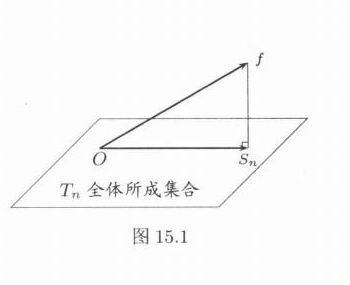
\includegraphics[width=.42\linewidth]{figures/lower/ch15/fig-15-1.png}
\end{center}

由命题 15.1.6 还可以得到

\begin{xproposition}[15.1.7（Bessel 不等式）]
若 $f$ 于区间 $[-\pi,\pi]$ 上可积和平方可积，且
\[
  f(x)\sim\frac{a_0}{2}+\sum_{n=1}^{\infty}(a_n\cos nx+b_n\sin nx),
\]
则有
\begin{equation}
  \frac{a_0^2}{2}+\sum_{n=1}^{\infty}(a_n^2+b_n^2)
  \le\frac1\pi\int_{-\pi}^{\pi}f^2(x)\,\dd x.
  \tag{15.11}
  \label{eq:15.11}
\end{equation}
\end{xproposition}

\begin{xproof}
从命题 15.1.6 得到
\[
  2\pi d^2(f,S_n)=\int_{-\pi}^{\pi}f^2\,\dd x-\frac{\pi a_0^2}{2}-\pi\sum_{k=1}^{n}(a_k^2+b_k^2)\ge0.
\]
由于这对每个 $n$ 成立，因此 (15.11) 左边的正项级数的每个部分和均以右边的积分为上界，从而收敛，且使该不等式成立。
\end{xproof}

\begin{xremark}
这个结果与 Fourier 级数的收敛性没有关系，由此就可以得到 $a_n=\littleo(1),b_n=\littleo(1)$，这里也不需要用 Riemann 引理。
\end{xremark}

\begin{xremark}
由此可知，在 $0<p\le1/2$ 时，三角级数
\[
  \sum_{n=1}^{\infty}\frac{\sin nx}{n^p},\qquad
  \sum_{n=1}^{\infty}\frac{\cos nx}{n^p}
\]
不可能是可积和平方可积函数的 Fourier 级数\footnote{但是这两个三角级数仍然是其和函数的 Fourier 级数，它们的和函数不平方可积，但可积和绝对可积。见后面的例题 15.2.3 和 15.2.4。}。
\end{xremark}

\subsection{例题}

\begin{xexample}[15.1.1]
证明：三角多项式
\[
  P_n(x)=\sum_{k=0}^{n}(A_k\cos kx+B_k\sin kx)
\]
的 Fourier 级数就是其本身。
\end{xexample}
\begin{xproof}
三角多项式可看成是只含有限个非零项的三角级数，因此在 $(-\infty,+\infty)$ 上一致收敛，引用命题 15.1.1 即得。（本题的另一个解法当然是直接计算。）
\end{xproof}

在用公式计算 Fourier 系数时，即使对于相当简单的 $f$，也可能要作多次分部积分运算，计算量相当大。因此，除了要细心地按公式计算之外，还应该学习（或发明）一些较为灵活的计算方法。为此在下面列举几种非常规方法供参考。此外，在学了逐项积分定理后还会有新的计算方法。

\begin{xexample}[15.1.2]
设函数 $f(x)=x^3,\ x\in(-\pi,\pi)$，求 $f$ 的 Fourier 级数。
\end{xexample}
\begin{xsolution}
\textbf{解 1}\quad 利用 Euler 公式 $\ee^{\ii\theta}=\cos\theta+\ii\sin\theta$ 在复数域进行计算往往是很有效的方法。对本题可以计算如下：
\begin{align*}
  \frac1\pi\int_{-\pi}^{\pi}x^3(\cos nx+\ii\sin nx)\,\dd x
  &=\frac1\pi\int_{-\pi}^{\pi}x^3\ee^{\ii nx}\,\dd x\\
  &=\frac1\pi\left(
    \frac{x^3}{\ii n}\ee^{\ii nx}
    -\frac{3x^2}{(\ii n)^2}\ee^{\ii nx}
    +\frac{6x}{(\ii n)^3}\ee^{\ii nx}
    -\frac6{(\ii n)^4}\ee^{\ii nx}
  \right)_{-\pi}^{\pi}\\
  &=\ii\,\frac{2(-1)^n}{\pi}\left(-\frac{\pi^3}{n}+\frac{6\pi}{n^3}\right)
   =\ii(-1)^{n-1}\left(\frac{2\pi^2}{n}-\frac{12}{n^3}\right).
\end{align*}
于是所求的 Fourier 级数为
\[
  \sum_{n=1}^{\infty}(-1)^{n-1}\left(\frac{2\pi^2}{n}-\frac{12}{n^3}\right)\sin nx.
\]

\textbf{解 2}\quad 这里的工具是命题 15.1.2。先用公式 (15.2) 直接计算出在 $(-\pi,\pi)$ 上函数 $x$ 的 Fourier 级数：
\begin{equation}
  x\sim\sum_{n=1}^{\infty}\frac{2(-1)^{n-1}}{n}\sin nx,
  \tag{15.12}
  \label{eq:15.12}
\end{equation}
然后从 $(x^2)'=2x$ 和公式 (15.6) 得到
\begin{equation}
  x^2\sim\frac{\pi^2}{3}+\sum_{n=1}^{\infty}\frac{4(-1)^n}{n^2}\cos nx,
  \tag{15.13}
  \label{eq:15.13}
\end{equation}
其中常数项是直接计算得到的。

由于在区间 $(-\pi,\pi)$ 上的 $x^3$ 不可能连续延拓为周期 $2\pi$ 的连续函数，因此不能直接用命题 15.1.2，但可以采用技巧 (15.7) 将 $x^3$ 分解为：
\begin{equation}
  x^3=(x^3-\pi^2x)+\pi^2x.
  \tag{15.14}
  \label{eq:15.14}
\end{equation}
右边第一项可以延拓为满足命题 15.1.2 的周期 $2\pi$ 的连续函数，其导函数为 $3x^2-\pi^2$，因此就可以用公式 (15.6) 和 (15.12) 得到 $x^3$ 的正弦级数中 $\sin nx$ 的系数为
\[
  3\cdot\frac{4(-1)^n}{n^3}+\pi^2\cdot\frac{2(-1)^{n-1}}{n}
  =\frac{(-1)^n12}{n^3}+\frac{(-1)^{n-1}2\pi^2}{n}.
\]
\end{xsolution}

\begin{xexample}[15.1.3]
设 $f$ 为 $(0,\pi/2)$ 上的可积和绝对可积函数。问：如何将 $f$ 延拓到区间 $(-\pi,\pi)$ 上，使其 Fourier 级数具有如下的形式：
\[
  \sum_{n=1}^{\infty}a_{2n-1}\cos(2n-1)x.
\]
\end{xexample}
\begin{xsolution}
由题意要求 $a_{2n}=0$，从公式
\[
  a_{2n}=\frac2\pi\int_0^{\pi}f(x)\cos2nx\,\dd x
\]
可见，由于 $\cos2nx$ 在 $[0,\pi]$ 上关于其中点为偶函数，根据上册 324 页命题 10.4.5，只要有 $f(x)=-f(\pi-x)$ 成立即可以使上述积分为 0。这决定了 $f$ 在 $(\pi/2,\pi)$ 上的延拓。定义 $f(0)=f(\pi/2)=0$，然后用偶延拓 $f(-x)=f(x)$ 将 $f$ 延拓到 $(-\pi,0)$ 上即可。

结论：将 $f$ 以如下方式延拓：
\[
  F(x)=
  \begin{cases}
    f(x),&x\in(0,\pi/2),\\
    -f(\pi-x),&x\in(\pi/2,\pi),\\
    0,&x=0,\pi/2,\\
    f(-x),&x\in(-\pi,0).
  \end{cases}
\]
\end{xsolution}

\subsection{练习题}

\begin{xexercise}[1]
求下列函数的 Fourier 级数：
  \begin{enumerate}[label=(\arabic*)]
    \item $\sin^3x+\cos^4x$；
    \item $ax^3+bx^2+cx+d,\ x\in(-\pi,\pi)$。
  \end{enumerate}
\end{xexercise}
\begin{xsolution}
(1) 利用恒等式
\[
  \sin^3x=\frac{3\sin x-\sin3x}{4},\qquad
  \cos^4x=\frac{3+4\cos2x+\cos4x}{8},
\]
得到
\[
  \sin^3x+\cos^4x
  =\frac38+\frac12\cos2x+\frac18\cos4x
   +\frac34\sin x-\frac14\sin3x.
\]
右边本身就是有限三角多项式，故即为所求 Fourier 级数。

(2) 在 $(-\pi,\pi)$ 上已有
\[
  x\sim2\sum_{n=1}^{\infty}\frac{(-1)^{n-1}}n\sin nx,
\]
\[
  x^2\sim\frac{\pi^2}{3}+4\sum_{n=1}^{\infty}\frac{(-1)^n}{n^2}\cos nx,
\]
以及
\[
  x^3\sim\sum_{n=1}^{\infty}(-1)^{n-1}
  \left(\frac{2\pi^2}{n}-\frac{12}{n^3}\right)\sin nx.
\]
因此线性组合给出
\begin{align*}
  ax^3+bx^2+cx+d
  &\sim \frac{b\pi^2}{3}+d
   +4b\sum_{n=1}^{\infty}\frac{(-1)^n}{n^2}\cos nx\\
  &\quad+
  \sum_{n=1}^{\infty}(-1)^{n-1}
  \left(\frac{2a\pi^2+2c}{n}-\frac{12a}{n^3}\right)\sin nx.
\end{align*}
该函数在 $(-\pi,\pi)$ 内光滑，所以 Fourier 级数在每个 $x\in(-\pi,\pi)$ 收敛于原函数；在端点处收敛于周期延拓的左右极限平均值。
\end{xsolution}


\begin{xexercise}[2]
将定义在 $(0,\pi/2)$ 上的可积和绝对可积函数 $f$ 延拓到区间 $(-\pi,\pi)$ 上，使其 Fourier 级数具有如下的形式：
  \[
    \sum_{n=1}^{\infty}b_{2n-1}\sin(2n-1)x.
  \]
\end{xexercise}
\begin{xsolution}
要使展开式只含奇数阶正弦项，先作奇延拓以消去全部余弦项，再令正弦系数中的偶数项消失。

在 $(0,\pi)$ 上定义
\[
  F(x)=
  \begin{cases}
    f(x),&0<x<\pi/2,\\
    f(\pi-x),&\pi/2<x<\pi,
  \end{cases}
\]
并取端点值任意，例如 $F(0)=F(\pi/2)=F(\pi)=0$；再在 $(-\pi,0)$ 上令
\[
  F(-x)=-F(x).
\]
于是 $F$ 为奇函数，所以 $a_n=0$。又对偶数指标 $2m$，
\begin{align*}
  b_{2m}
  &=\frac2\pi\int_0^\pi F(x)\sin2mx\,\dd x\\
  &=\frac2\pi\int_0^{\pi/2}
  \bigl[F(x)\sin2mx+F(\pi-x)\sin(2m(\pi-x))\bigr]\,\dd x=0,
\end{align*}
因为 $F(\pi-x)=F(x)$ 而
$\sin(2m(\pi-x))=-\sin2mx$。故 Fourier 级数只有
\[
  \sum_{m=1}^{\infty}b_{2m-1}\sin(2m-1)x
\]
中的项。
\end{xsolution}


\begin{xexercise}[3]
证明：函数
  \[
    f(x)=\begin{cases}
      c,&0<x\le\pi,\\
      0,&x=0,\\
      -c,&-\pi<x<0
    \end{cases}
  \]
  的 Fourier 级数的前 $2n+1$ 项的和
  \[
    S_n(x)=\frac{a_0}{2}+\sum_{k=1}^{n}(a_k\cos kx+b_k\sin kx)
  \]
  具有形式
  \[
    S_n(x)=\frac{2c}{\pi}\int_0^x\frac{\sin2nt}{\sin t}\,\dd t.
  \]
\end{xexercise}
\begin{xsolution}
函数为奇函数，故 $a_n=0$。对 $k\ge1$，
\[
  b_k=\frac2\pi\int_0^\pi c\sin kx\,\dd x
  =\frac{2c}{\pi k}\bigl(1-(-1)^k\bigr).
\]
于是
\[
  b_{2j}=0,\qquad b_{2j-1}=\frac{4c}{\pi(2j-1)}.
\]
因此标准 Fourier 部分和满足
\[
  S_{2m-1}(x)=S_{2m}(x)
  =\frac{4c}{\pi}\sum_{j=1}^{m}\frac{\sin(2j-1)x}{2j-1}.
\]
另一方面有恒等式
\[
  \frac{\sin2mt}{\sin t}=2\sum_{j=1}^{m}\cos(2j-1)t.
\]
从 $0$ 到 $x$ 积分即得
\[
  \frac{2c}{\pi}\int_0^x\frac{\sin2mt}{\sin t}\,\dd t
  =\frac{4c}{\pi}\sum_{j=1}^{m}\frac{\sin(2j-1)x}{2j-1}.
\]
故可核验的关系为
\[
  \boxed{\displaystyle
  S_{2m-1}(x)=S_{2m}(x)
  =\frac{2c}{\pi}\int_0^x\frac{\sin2mt}{\sin t}\,\dd t }.
\]
原题若把右端的 $m$ 仍记作 $n$，则左端应相应写成 $S_{2n-1}$ 或 $S_{2n}$。
\end{xsolution}


\begin{xexercise}[4]
设 $f\in C^1[-\pi,\pi]$，证明：
  \[
    a_n=\littleo\!\left(\frac1n\right),\qquad b_n=\bigO\!\left(\frac1n\right);
  \]
  如果又有 $f(\pi)=f(-\pi)$，则 $b_n=\littleo(1/n)$。
\end{xexercise}
\begin{xsolution}
由分部积分，
\begin{align*}
  a_n
  &=\frac1\pi\int_{-\pi}^{\pi}f(x)\cos nx\,\dd x
   =-\frac1{n\pi}\int_{-\pi}^{\pi}f'(x)\sin nx\,\dd x.
\end{align*}
因为 $f'$ 连续，Riemann 引理给出
\[
  \int_{-\pi}^{\pi}f'(x)\sin nx\,\dd x=\littleo(1),
\]
故
\[
  a_n=\littleo\!\left(\frac1n\right).
\]
同理
\begin{align*}
  b_n
  &=\frac1\pi\int_{-\pi}^{\pi}f(x)\sin nx\,\dd x\\
  &=-\frac{(-1)^n}{n\pi}\bigl[f(\pi)-f(-\pi)\bigr]
    +\frac1{n\pi}\int_{-\pi}^{\pi}f'(x)\cos nx\,\dd x.
\end{align*}
第二项为 $\littleo(1/n)$，第一项为 $\bigO(1/n)$，所以
\[
  b_n=\bigO\!\left(\frac1n\right).
\]
若再有 $f(\pi)=f(-\pi)$，边界项消失，从而
\[
  b_n=\littleo\!\left(\frac1n\right).
\]
\end{xsolution}


\begin{xexercise}[5]
设 $f$ 是以 $2\pi$ 为周期的有界函数且在 $(-\pi,\pi)$ 上逐段单调，证明：
  \[
    a_n=\bigO\!\left(\frac1n\right),\qquad b_n=\bigO\!\left(\frac1n\right).
  \]
  （可在每个单调区间上用积分第二中值定理（见上册的命题 10.2.2）。）
\end{xexercise}
\begin{xsolution}
设 $(-\pi,\pi)$ 被有限个点分成若干单调区间 $I_j=[\alpha_j,\beta_j]$，并设
$\abs{f(x)}\le M$。只需在每个 $I_j$ 上估计振荡积分。

若 $f$ 在 $I_j$ 上单调，由积分第二中值定理，存在 $\xi_j\in I_j$，使
\[
  \int_{\alpha_j}^{\beta_j}f(x)\cos nx\,\dd x
  =f(\alpha_j+)\int_{\alpha_j}^{\xi_j}\cos nx\,\dd x
   +f(\beta_j-)\int_{\xi_j}^{\beta_j}\cos nx\,\dd x.
\]
每个余弦积分的绝对值不超过 $2/n$，故
\[
  \left|\int_{\alpha_j}^{\beta_j}f(x)\cos nx\,\dd x\right|
  \le\frac{4M}{n}.
\]
单调区间数有限，求和即得
\[
  a_n=\bigO\!\left(\frac1n\right).
\]
对正弦积分，在每个 $I_j$ 上再次用积分第二中值定理，可写成两个形如
\[
  f(\alpha_j+)\int_{\alpha_j}^{\eta_j}\sin nx\,\dd x,
  \qquad
  f(\beta_j-)\int_{\eta_j}^{\beta_j}\sin nx\,\dd x
\]
的项；每个正弦积分的绝对值也不超过 $2/n$。因此逐段求和后
\[
  b_n=\bigO\!\left(\frac1n\right).
\]
\end{xsolution}


\begin{xexercise}[6]
设 $f$ 是以 $2\pi$ 为周期的函数且在 $[-\pi,\pi]$ 上可积和绝对可积，证明：用 $\sin x$ 去乘 $f$ 的 Fourier 级数的每一项所得的三角级数就是 $f(x)\sin x$ 的 Fourier 级数。
\end{xexercise}
\begin{xsolution}
设
\[
  f(x)\sim\frac{a_0}{2}+\sum_{n=1}^{\infty}(a_n\cos nx+b_n\sin nx),
\]
并约定 $b_0=0$。令 $g(x)=f(x)\sin x$。利用积化和差公式，对 $m\ge1$ 有
\begin{align*}
  A_m
  &=\frac1\pi\int_{-\pi}^{\pi}g(x)\cos mx\,\dd x\\
  &=\frac1{2\pi}\int_{-\pi}^{\pi}f(x)
    \bigl[\sin(m+1)x-\sin(m-1)x\bigr]\,\dd x\\
  &=\frac{b_{m+1}-b_{m-1}}2,
\end{align*}
而
\begin{align*}
  B_m
  &=\frac1\pi\int_{-\pi}^{\pi}g(x)\sin mx\,\dd x\\
  &=\frac1{2\pi}\int_{-\pi}^{\pi}f(x)
    \bigl[\cos(m-1)x-\cos(m+1)x\bigr]\,\dd x\\
  &=\frac{a_{m-1}-a_{m+1}}2,
\end{align*}
其中 $m=1$ 时 $a_{m-1}=a_0$。此外
\[
  A_0=\frac1\pi\int_{-\pi}^{\pi}f(x)\sin x\,\dd x=b_1.
\]
另一方面，形式上逐项乘以 $\sin x$ 后
\begin{align*}
  \sin x\left[\frac{a_0}{2}+\sum_{n\ge1}(a_n\cos nx+b_n\sin nx)\right]
\end{align*}
用同样的积化和差公式整理，恰好得到常数项 $A_0/2$、余弦系数 $A_m$ 与正弦系数 $B_m$。因此所得三角级数正是 $f(x)\sin x$ 的 Fourier 级数。
\end{xsolution}


\begin{xexercise}[7]
设 $[a,b]$ 上的连续函数系 $\{e_n\}$ 满足条件
  \[
    \int_a^b e_i(x)e_j(x)\,\dd x=\delta_{ij},
  \]
  其中 $\delta_{ij}=0,\ \forall i\ne j$，$\delta_{ii}=1$，则称该函数系在 $[a,b]$ 上为规范正交系。设 $f$ 在 $[a,b]$ 上可积和平方可积，定义
  \[
    c_n=\int_a^b f(x)e_n(x)\,\dd x
  \]
  为 $f$ 关于 $e_n$ 的 Fourier 系数，$n=1,2,\ldots$。证明：级数 $\sum_{n=1}^{\infty}c_n^2$ 收敛。又问：当 $n$ 固定时，$a_1,a_2,\ldots,a_n$ 取什么值时，平方平均误差
  \[
    \int_a^b\left[f(x)-\sum_{k=1}^{n}a_ke_k(x)\right]^2\,\dd x
  \]
  最小？
\end{xexercise}
\begin{xsolution}
令
\[
  E_n(a_1,\ldots,a_n)
  =\int_a^b\left[f(x)-\sum_{k=1}^{n}a_ke_k(x)\right]^2\,\dd x.
\]
利用规范正交性，展开得
\begin{align*}
  E_n
  &=\int_a^bf^2(x)\,\dd x
    -2\sum_{k=1}^{n}a_kc_k+\sum_{k=1}^{n}a_k^2\\
  &=\int_a^bf^2(x)\,\dd x-\sum_{k=1}^{n}c_k^2
    +\sum_{k=1}^{n}(a_k-c_k)^2.
\end{align*}
因为 $E_n\ge0$，取 $a_k=c_k$ 即得 Bessel 不等式
\[
  \sum_{k=1}^{n}c_k^2\le\int_a^bf^2(x)\,\dd x.
\]
左端随 $n$ 单调增加且有统一上界，故
\[
  \sum_{n=1}^{\infty}c_n^2
\]
收敛。

同时上面的配方公式说明，当 $n$ 固定时，$E_n$ 的唯一最小值在
\[
  \boxed{a_k=c_k\quad(k=1,\ldots,n)}
\]
处取得。
\end{xsolution}


\begin{xexercise}[8]
设 $g$ 是周期为 1 的连续函数且 $\int_0^1g(x)\,\dd x=0$，函数 $f\in C^1[0,1]$，令
  \[
    a_n=\int_0^1f(x)g(nx)\,\dd x,\quad n=1,2,\ldots,
  \]
  证明：级数 $\sum_{n=1}^{\infty}a_n^2$ 收敛。
\end{xexercise}
\begin{xsolution}
令
\[
  G(x)=\int_0^xg(t)\,\dd t.
\]
由于 $g$ 的周期为 $1$ 且 $\int_0^1g=0$，有 $G(x+1)=G(x)$，所以 $G$ 连续且有界。又
\[
  \frac{\dd}{\dd x}G(nx)=n g(nx).
\]
因此分部积分给出
\begin{align*}
  a_n
  &=\frac1n\int_0^1f(x)\,\dd[G(nx)]\\
  &=\frac1n\bigl[f(x)G(nx)\bigr]_0^1
    -\frac1n\int_0^1f'(x)G(nx)\,\dd x.
\end{align*}
取 $G(0)=0$，则 $G(n)=G(0)=0$，边界项为零。若
$\norm{G}_\infty=M$，则
\[
  \abs{a_n}\le\frac{M}{n}\int_0^1\abs{f'(x)}\,\dd x=\bigO\!\left(\frac1n\right).
\]
于是
\[
  \sum_{n=1}^{\infty}a_n^2
\]
由与 $\sum1/n^2$ 比较而收敛。
\end{xsolution}


\section{Fourier 级数的收敛性}

本节讨论 Fourier 级数在各种意义上的收敛性问题，其中包括点收敛，在 Cesàro 意义下的收敛，平方平均收敛和一致收敛。

为了方便起见，在以下的叙述中只考虑周期 $2\pi$ 的情况，但通过简单变换就可以将结论推广到一般周期的情况。

\subsection{Dirichlet 核和点收敛性}

Fourier 级数的点收敛性研究主要依赖于 Dirichlet 核（参见上册 322 页）。利用 Euler-Fourier 公式和三角变换，将函数 $f$ 的 Fourier 级数的部分和函数列
\[
  S_0(x)=\frac{a_0}{2},\qquad
  S_n(x)=\frac{a_0}{2}+\sum_{k=1}^{n}(a_k\cos kx+b_k\sin kx),\quad n=1,2,\ldots,
\]
用 Dirichlet 积分表示出来：
\begin{equation}
  S_n(x)=\frac1\pi\int_{-\pi}^{\pi}f(x+t)D_n(t)\,\dd t
  =\frac1\pi\int_0^{\pi}[f(x+t)+f(x-t)]D_n(t)\,\dd t,
  \tag{15.15}
  \label{eq:15.15}
\end{equation}
其中 $D_n$ 是 Dirichlet 核
\begin{equation}
  D_n(x)=\frac12+\sum_{k=1}^{n}\cos kx
  =\frac{\sin(n+\frac12)x}{2\sin\frac x2}.
  \tag{15.16}
  \label{eq:15.16}
\end{equation}
$D_n(x)$ 是周期为 $2\pi$ 的函数，在一个周期上的积分值为 $\pi$（见上册 (10.12)）：
\begin{equation}
  \frac2\pi\int_0^{\pi}D_n(x)\,\dd x=1.
  \tag{15.17}
  \label{eq:15.17}
\end{equation}
从方法上观察，局部化定理以及各种常见判别法都可以通过对 Dirichlet 核的研究而得到。在图 15.2 中作出了 $D_n(x)$ 在区间 $[-\pi,\pi]$ 上的示意图，其中取 $n=9$。$x=0$ 为 $D_n(x)$ 的可去间断点，其极限值为 $n+\frac12$，是曲线的主峰高度。$D_n(x)$ 的绝对值最小的两个零点 $\pm\pi/(n+\frac12)$ 之间的主峰下的面积当 $n\to\infty$ 时趋于 $\pi$，而其余峰谷和横轴之间的面积之和则正负相消趋于 0。因此公式 (15.17) 中的积分值主要就是由这个最高的主峰提供的。

$D_n(x)$ 的这些特性使得当函数 $g(x)$ 在 $x=0$ 处满足一定条件（例如可导）时，就能够建立
\[
  \lim_{n\to\infty}\frac1\pi\int_{-\pi}^{\pi}D_n(x)g(x)\,\dd x=g(0).
\]
这就是 Dirichlet 核的作用，即通过积分运算和取极限“提取”出函数 $g$ 在 $x=0$ 的值。若对 $g$ 的自变量作平移就可以得到其他点的值。

由此得到的第一个结果就是局部化定理，它是 Fourier 级数的一个特点。由于函数 $f$ 的 Fourier 系数是按照 Euler-Fourier 公式通过积分得到的，因此 $f$ 的 Fourier 级数在点 $x_0$ 处的敛散性似乎理所当然地应当与 $f$ 在整个区间 $[-\pi,\pi]$ 上的性态有关。但局部化定理对此给出了完全不同的论断。有关点收敛的各种判别法也都是在这个基础上建立起来的。

\begin{center}
  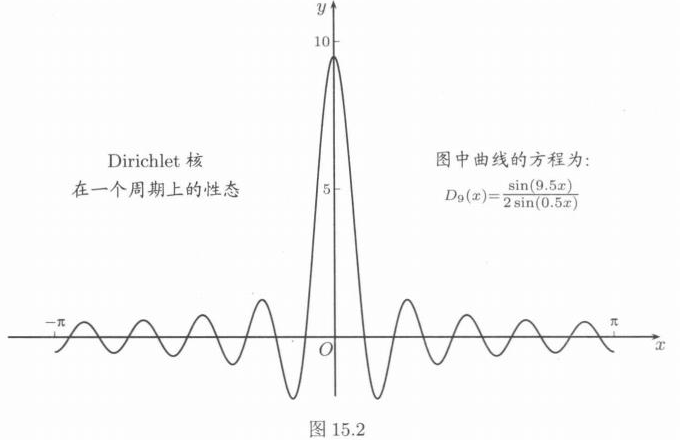
\includegraphics[width=.74\linewidth]{figures/lower/ch15/fig-15-2.png}
\end{center}

局部化定理即是对任意小的固定正数 $\delta$ 有渐近等式：
\[
  S_n(x)=\frac1\pi\int_0^{\delta}[f(x+t)+f(x-t)]D_n(t)\,\dd t+\littleo(1)\qquad(n\to\infty).
\]
利用 (15.17)，对于任意 $s$ 就有
\begin{equation}
  S_n(x)-s=\frac1\pi\int_0^{\pi}[f(x+t)+f(x-t)-2s]D_n(t)\,\dd t.
  \tag{15.18}
  \label{eq:15.18}
\end{equation}
这样就可以研究在什么条件下 $f$ 的 Fourier 级数于点 $x$ 处收敛于 $s$。由于 (15.18) 的特殊形式，经常令
\[
  s=\frac12[f(x^+)+f(x^-)],
\]
并在一系列条件下证明 $f$ 的 Fourier 级数收敛于这个值。这就是教科书中的一系列判别法，当然它们都是充分性判别法。本书在这里不再重复。

需要指出，Fourier 级数的点收敛性是一个十分困难的问题，即使对于连续周期函数也是如此。这里浏览一下已经取得的进展是适宜的。

\paragraph{Fourier 级数的点收敛的研究进展}
早期进展是举出发散的例子。要找到一个连续函数，使得它的 Fourier 级数在一个点上发散，这已经不是一个平凡的问题。自从 Du Bois-Reymond（1873）举出了这样的例子之后，发散点处处稠密的连续函数例子也已经找到。若在 Lebesgue 可积函数类中考虑问题，则 Kolmogorov（柯尔莫哥洛夫）举出了 $f$ 的 Fourier 级数几乎处处发散（1923）和处处发散（1926）的例子。（几乎处处是实变函数论中的概念，在上册 304 页已有解释。）

另一方面，Lusin（卢津）则猜测连续函数的 Fourier 级数几乎处处收敛。由于以上所举出的各反例，在很长的时间内很少有人相信这个猜测是正确的。这个猜测最终在 1966 年为 Carleson（卡勒松）正面解决，他证明了包含连续函数在内的 $L$ 平方可积函数的 Fourier 级数一定是几乎处处收敛的。这是一个引起轰动的重大成果。（Carleson 是 1992 年 Wolf（沃尔夫）奖的获得者。）

\subsection{Gibbs 现象}

由于 Fourier 级数的每一项是连续函数，因此容易知道，如果 Fourier 级数的和函数在某点不连续，则级数在该点的邻域上不可能是一致收敛的。但是对于 Fourier 级数来说这里还有一个更为奇特的现象，即所谓 Gibbs（吉布斯）现象。这里的要点是：若 $x_0$ 是和函数的一个（第一类）间断点，则当 $x_n$ 趋于 $x_0$ 的左侧或右侧时，部分和的值 $S_n(x_n)$ 不会收敛于 $S(x_0)$。不但如此，下面的分析表明，这里的误差不会因 $n$ 的增加而减小。

为简单起见，我们先讨论具有典型意义的一个特例：
\begin{equation}
  S(x)=\sum_{n=1}^{\infty}\frac{\sin nx}{n},
  \tag{15.19}
  \label{eq:15.19}
\end{equation}
其中 $S(x)$ 是周期 $2\pi$ 的函数：
\[
  S(x)=\frac{\pi-x}{2},\quad \forall x\in(0,2\pi),\qquad S(0)=0.
\]
在图 15.3 中作出了级数 (15.19) 的前 10 个部分和函数的示意图。

\begin{center}
  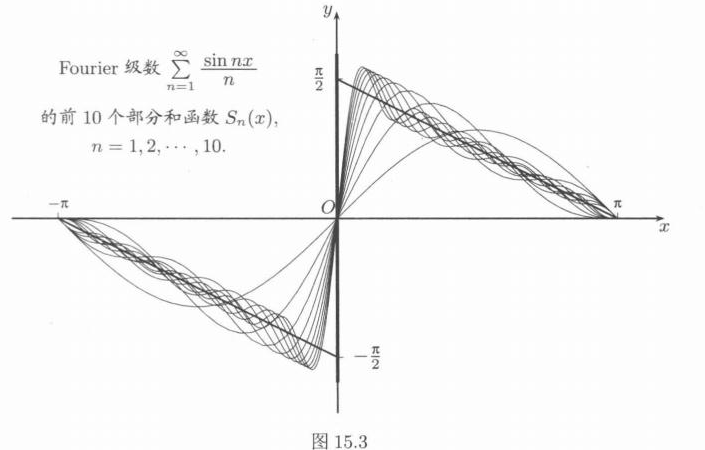
\includegraphics[width=.75\linewidth]{figures/lower/ch15/fig-15-3.png}
\end{center}

同时在图 15.3 中还用两段粗黑直线表示级数 (15.19) 的和函数
\[
  S(x)=\frac{\pi-x}{2},\qquad x\in[-\pi,0)\cup(0,\pi].
\]
从图中已经可以看出，虽然只观察了前 10 个部分和函数，但在点 $x=0$ 附近的差值 $\abs{S_n(x)-S(x)}$ 毫无趋于 0 的趋势，更为精确的性态刻画可以总结如下。（其中只叙述 $0\le x\le\pi$ 的情况，对 $-\pi\le x\le0$ 的结论是类似的。）

\begin{xexample}[15.2.1（Gibbs 现象）]
记 $\{S_n(x)\}$ 是 Fourier 级数 (15.19) 的部分和函数列，$S(x)=(\pi-x)/2$ 为该级数在区间 $(0,2\pi)$ 上的和函数，则有
\[
  \lim_{n\to\infty}\max_{0\le x\le\pi}\{S_n(x)-S(x)\}
  =\int_0^{\pi}\frac{\sin t}{t}\,\dd t-\frac\pi2
  \approx\frac\pi2\times0.17898.
\]
\end{xexample}
\begin{xproof}
研究误差 $\varepsilon_n(x)=S_n(x)-S(x)$ 在 $x=0$ 右侧的性态。直接计算得到
\[
  \frac{\dd\varepsilon_n(x)}{\dd x}=\frac12+\sum_{k=1}^{n}\cos kx,
\]
因此就有（见前面的 (15.16)）
\[
  \frac{\dd\varepsilon_n(x)}{\dd x}=D_n(x)=\frac{\sin(n+\frac12)x}{2\sin\frac12x}.
\]
可以看出误差 $\varepsilon_n(x)$ 的极值点为
\[
  x_n^{(m)}=\frac{\pi m}{n+\frac12},\qquad m=1,2,\ldots,2n.
\]
其中当 $m$ 为奇数时是极大值点\footnote{可以证明 $\max_{0\le x\le\pi}\{S_n(x)-S(x)\}=\varepsilon_n(x_n^{(1)})$，例如参考 [18] 第三卷的 700--701 小节。}，当 $m$ 为偶数时是极小值点（参见图 15.3）。

直接计算在这些极值点上的误差值：
\begin{align*}
  \varepsilon_n(x_n^{(m)})
  &=S_n(x_n^{(m)})-S(x_n^{(m)})
   =\sum_{k=1}^{n}\frac{\sin(kx_n^{(m)})}{k}-\frac{\pi-x_n^{(m)}}2\\
  &=\left(\sum_{k=1}^{n}\frac{\sin(kx_n^{(m)})}{kx_n^{(m)}}\cdot\frac{\pi m}{n}\right)
    \left(\frac{n}{n+1/2}\right)-\frac\pi2+\frac{\pi m}{2n+1}\\
  &=\left(\sum_{k=1}^{n}\frac{\sin(kx_n^{(m)})}{kx_n^{(m)}}\cdot\frac{\pi m}{n}\right)-\frac\pi2+\bigO\!\left(\frac1n\right).
\end{align*}
由于右边第一项可看作为 Riemann 积分和式，因此当 $n\to\infty$ 时就得到
\[
  \lim_{n\to\infty}\varepsilon_n(x_n^{(m)})=\int_0^{\pi m}\frac{\sin t}{t}\,\dd t-\frac\pi2.
\]
容易知道当 $m=1$ 时的极限值最大\footnote{不难证明变上限积分 $\int_0^x(\sin t/t)\,\dd t$ 的最大值也就是在 $x=\pi$ 处达到。}，即得到
\[
  \int_0^{\pi}\frac{\sin t}{t}\,\dd t-\frac\pi2\approx\frac\pi2\times0.17898.
\]
\end{xproof}

\begin{xremark}
若取 $x_n=c/n,\ n=1,2,\ldots$，则类似地有
\[
  \lim_{n\to\infty}S_n\left(\frac cn\right)=\int_0^c\frac{\sin t}{t}\,\dd t.
\]
取不同的 $c$ 值，这样的极限值就会形成一个闭区间 $[CS(0^-),CS(0^+)]$，其中
\[
  C=\frac2\pi\int_0^{\pi}\frac{\sin t}{t}\,\dd t\approx1.17898.
\]
注意：在图 15.3 上用 $y$ 轴上的一个粗黑直线段来代表这个区间。
\end{xremark}

\begin{xremark}
虽然以上只是一个特例，但可以用它以及它的平移来吸收一般的和函数中的所有间断点。因此以上所得的结论、常数 18\% 以及注 1 中的内容都具有普遍意义。
\end{xremark}

\paragraph{小结}
若和函数有间断点，则不可能依靠 Fourier 级数的部分和函数 $S_n(x)$ 的 $n$ 增加来改进近似计算的精确程度。这是在 Fourier 级数的应用中不能忽视的问题（可以参考 [43] 的最后一章“三角级数之和”）。

\begin{xremark}
以上证明的思想来自《美国数学月刊》(1980) 第 87 卷 210--212 页。
\end{xremark}

\subsection{Fourier 级数的 Cesàro 求和}

到目前为止，凡是说到无穷级数 $\sum_{n=0}^{\infty}a_n$ 收敛，就是指它的部分和数列收敛。这就是由 Cauchy 提出的无穷级数的收敛定义，但至少从 Euler 起，就已经出现无穷级数的其他收敛定义。Cesàro 求和就是其中的一种，它在 Fourier 级数理论中得到了重要的应用（参见第十三章最后的几个参考题）。

\paragraph{定义}
设级数 $\sum_{n=0}^{\infty}a_n$ 的部分和数列为
\[
  S_n=a_0+a_1+\cdots+a_n,\qquad n=0,1,2,\ldots.
\]
定义数列
\[
  \sigma_n=\frac{S_0+S_1+\cdots+S_{n-1}}{n},\qquad n=1,2,\ldots.
\]
如果存在极限 $\lim_{n\to\infty}\sigma_n=\sigma$，则称级数 $\sum_{n=0}^{\infty}a_n$ 在 Cesàro 意义下可求和，且定义 $\sigma$ 为级数 $\sum_{n=0}^{\infty}a_n$ 的 Cesàro 和。由 Cauchy 命题（见上册 31 页）知道，若数列 $\{S_n\}$ 收敛于数 $S$，则其前 $n$ 项的平均值 $\sigma_n$ 构成的数列也收敛于 $S$，但反之则不然。因此若级数 $\sum a_n$ 在通常意义下收敛，则它在 Cesàro 意义下也收敛，且有相同的和。这表明对于在通常意义下收敛的级数而言，Cesàro 求和没有给出新的结果。

然而在通常意义下的某些发散级数有可能在 Cesàro 意义下有和。例如级数
\[
  1-1+1-1+\cdots=\sum_{n=1}^{\infty}(-1)^{n-1}
\]
的部分和数列为 $S_{2k-1}=1,S_{2k}=0,\ k=1,2,\ldots$，因此该级数的 Cesàro 和为 $1/2$。这就是 Euler 等数学家曾经提出过的和（参见 [26,50]）。

初看起来这似乎有点荒谬，为什么要考虑（在通常意义下）发散级数的和？这样做有什么意义？下面我们先观察 Cesàro 求和在 Fourier 级数理论中给我们带来什么结果。

\begin{xproposition}[15.2.1（Fejér 定理）]
如果以 $2\pi$ 为周期的函数 $f$ 在 $[-\pi,\pi]$ 上可积和绝对可积，并且在点 $x_0$ 处有左、右极限 $f(x_0^+)$ 与 $f(x_0^-)$，则 $f$ 的 Fourier 级数在点 $x_0$ 处在 Cesàro 意义下收敛于
\[
  \frac12[f(x_0^+)+f(x_0^-)].
\]
特别是当 $f$ 于点 $x_0$ 连续时，则 Fourier 级数在点 $x_0$ 的 Cesàro 和就等于 $f(x_0)$。
\end{xproposition}

\begin{xproof}
从部分和函数列 $S_n(x)$ 的 Dirichlet 积分 (15.15) 出发计算 $\sigma_n(x)$，经三角变换后可以得到 Fejér 积分：
\[
  \sigma_n(x)=\frac1\pi\int_{-\pi}^{\pi}f(x+t)\cdot\frac1{2n}
  \left(\frac{\sin\frac n2t}{\sin\frac12t}\right)^2\,\dd t
  =\int_0^{\pi}\frac{f(x+t)+f(x-t)}2\,F_n(t)\,\dd t,
\]
其中的非负函数
\begin{equation}
  F_n(t)=\frac1{n\pi}\left(\frac{\sin\frac n2t}{\sin\frac12t}\right)^2
  \tag{15.20}
  \label{eq:15.20}
\end{equation}
称为 Fejér 核。用 $f(x)\equiv1$ 代入就得到恒等式（见上册 330 页的题 10）：
\begin{equation}
  \int_0^{\pi}F_n(t)\,\dd t=1.
  \tag{15.21}
  \label{eq:15.21}
\end{equation}
这样就可以利用 Fejér 积分和恒等式 (15.21) 将问题化为积分估计：
\[
  \left|\sigma_n(x_0)-\frac12[f(x_0^+)+f(x_0^-)]\right|
  \le\int_0^{\pi}
  \frac{\abs{f(x_0+t)-f(x_0^+)}+\abs{f(x_0-t)-f(x_0^-)}}2F_n(t)\,\dd t.
\]
现在对每个给定的 $\varepsilon>0$ 取 $\delta>0$，使得当 $0\le t\le\delta$ 时，有
\[
  \abs{f(x_0+t)-f(x_0^+)}<\varepsilon,
  \qquad
  \abs{f(x_0-t)-f(x_0^-)}<\varepsilon
\]
成立，于是就有
\[
  \int_0^{\delta}
  \frac{\abs{f(x_0+t)-f(x_0^+)}+\abs{f(x_0-t)-f(x_0^-)}}2F_n(t)\,\dd t
  \le\varepsilon\int_0^{\delta}F_n(t)\,\dd t\le\varepsilon,
\]
这里利用了 Fejér 核的非负性和恒等式 (15.21)。再利用当 $\delta\le t\le\pi$ 时
\[
  0\le F_n(t)\le\frac1{n\pi}\frac1{(\sin\frac12\delta)^2},
\]
就可以估计得到
\[
  \int_{\delta}^{\pi}
  \frac{\abs{f(x_0+t)-f(x_0^+)}+\abs{f(x_0-t)-f(x_0^-)}}2F_n(t)\,\dd t
  =\bigO\!\left(\frac1n\right).
\]
因此存在 $N$，使得当 $n>N$ 时有
\[
  \left|\sigma_n(x_0)-\frac12[f(x_0^+)+f(x_0^-)]\right|<2\varepsilon.
\]
这就是
\[
  \lim_{n\to\infty}\sigma_n(x_0)=\frac12[f(x_0^+)+f(x_0^-)].
\]
\end{xproof}

\begin{xremark}
将 Fejér 积分的估计和 Dirichlet 积分的估计作比较，可见这里要容易得多，连 Riemann 引理也不需要用。原因在于 Fejér 核是非负的，而 Dirichlet 核则是变号的（见图 15.2）。如前所示的 Gibbs 现象的根源都在于此。读者可以将图 15.4 中的 Fejér 核的示意图与图 15.2 作比较。此外，还可以参考 [18] 第三卷的 740 小节关于正核的系统论述。在下一章关于 Weierstrass 逼近定理的证明中我们将再次接触到这种核函数方法（又称奇异积分方法）。
\end{xremark}

由 Fejér 定理可以立即得到关于 Fourier 级数收敛的一个重要结果。

\begin{center}
  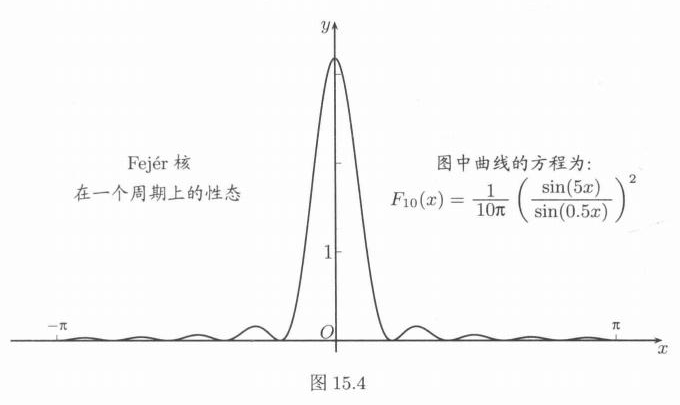
\includegraphics[width=.72\linewidth]{figures/lower/ch15/fig-15-4.png}
\end{center}

\begin{xproposition}[15.2.2]
设以 $2\pi$ 为周期的函数 $f$ 在 $[-\pi,\pi]$ 上可积和绝对可积，点 $x_0$ 是 $f$ 的连续点或第一类间断点，如果 $f$ 的 Fourier 级数在点 $x_0$ 处收敛，则它一定收敛于 $f(x_0)$ 或
\[
  \frac12[f(x_0^+)+f(x_0^-)].
\]
\end{xproposition}
\begin{xproof}
设 $f$ 的 Fourier 级数在点 $x_0$ 处收敛于 $s$，则其 Cesàro 和也是 $s$。但由 Fejér 定理（命题 15.2.1）可以知道它的 Cesàro 和为 $f(x_0)$ 或 $\frac12[f(x_0^+)+f(x_0^-)]$，可见命题成立。
\end{xproof}

\begin{xremark}
结合前面提到的 Carleson 的工作，可以知道连续周期函数的 Fourier 级数展开式一定几乎处处成立。
\end{xremark}

对于连续的周期函数，从 Fejér 定理还可以得到两个重要结论：

\begin{xproposition}[15.2.3（Fourier 级数的惟一性定理）]
设 $f$ 为周期 $2\pi$ 的连续函数，且其 Fourier 系数均等于 0：$a_0=0,a_n=b_n=0,\ n=1,2,\ldots$，则 $f$ 必是恒等于 0 的常值函数。
\end{xproposition}
\begin{xproof}
这时 $f$ 的 Fourier 级数的每一项都恒等于 0，因此部分和函数列 $\{S_n(x)\}$ 的每一项也都恒等于 0。由此就知道 $\sigma_n(x)\equiv0,\ n=1,2,\ldots$。从 Fejér 定理（命题 15.2.1）可见 $f\equiv0$。
\end{xproof}

\begin{xremark}
由此可知若两个连续函数有相同的 Fourier 系数，则这两个连续函数必相同。注意：这与 Taylor 级数很不一样（参见命题 14.4.2、67 页底注和上册 169 页的例题 6.2.4）。
\end{xremark}

\begin{xproposition}[15.2.4（关于一致收敛的 Fejér 定理）]
如果 $f$ 是以 $2\pi$ 为周期的连续函数，则它的 Fourier 级数在 Cesàro 意义下一致收敛于 $f$。
\end{xproposition}

\begin{xremark}
这只需要在命题 15.2.1 的证明中利用连续函数的 Cantor 定理（见上册 §5.4）即可。
\end{xremark}

\begin{xremark}
由于 $\{\sigma_n(x)\}$ 是三角多项式函数列，因此已经得到了关于周期连续函数用三角多项式一致逼近的 Weierstrass 第二逼近定理。这将在下一章中再作进一步介绍。（又见命题 15.2.8 的注和参考题 19。）
\end{xremark}

\subsection{Fourier 级数的平方平均收敛}

\paragraph{定义}
称函数列 $\{f_n\}$ 于区间 $[a,b]$ 上平方平均收敛于 $f$，若成立
\[
  \lim_{n\to\infty}\int_a^b\abs{f_n(x)-f(x)}^2\,\dd x=0.
\]
从 Bessel 不等式（即命题 15.1.7）的证明已知
\[
  2\pi d^2(f,S_n)=\int_{-\pi}^{\pi}f^2\,\dd x-\frac{\pi a_0^2}{2}-\pi\sum_{k=1}^{n}(a_k^2+b_k^2),
\]
因此，若 $\lim_{n\to\infty}d^2(f,S_n)=0$，则 Bessel 不等式中的不等号就可换为等号。这就是 Parseval（帕塞瓦尔）等式，它又称为封闭性方程，是 Fourier 级数中最重要的公式之一。

\begin{xproposition}[15.2.5（Parseval 等式）]
设 $f$ 在 $[-\pi,\pi]$ 上可积和平方可积，
\[
  f(x)\sim\frac{a_0}{2}+\sum_{n=1}^{\infty}(a_n\cos nx+b_n\sin nx),
\]
则有下列 Parseval 等式成立：
\begin{equation}
  \frac{a_0^2}{2}+\sum_{n=1}^{\infty}(a_n^2+b_n^2)
  =\frac1\pi\int_{-\pi}^{\pi}f^2(x)\,\dd x.
  \tag{15.22}
  \label{eq:15.22}
\end{equation}
\end{xproposition}

\begin{xproof}
这里只列出主要步骤，细节从略。
\begin{enumerate}[label=(\arabic*)]
  \item 先用连续函数在平方平均意义上逼近 $f$（参见上册 333 页题 5）。如果 $f$ 为广义平方可积，则还需要先用常义可积函数在平方平均意义上逼近 $f$，然后再用连续函数逼近。
  \item 对于连续函数，根据一致收敛的 Fejér 定理（即命题 15.2.4），存在一个三角多项式 $T_n$ 一致逼近这个连续函数。
  \item 然后再用 $S_n$ 在所有 $T_n$ 中的最优性（即命题 15.1.6），并注意到 $d^2(f,S_n)$ 随 $n$ 增大而单调减少，可见成立 $\lim_{n\to\infty}d^2(f,S_n)=0$，因此所求结论为真。
\end{enumerate}
\end{xproof}

\begin{xremark}
为了阐明 Parseval 等式的几何意义，只需要将函数空间中从正交开始的几何类比进一步做下去：将
\[
  \int_{-\pi}^{\pi}f(x)g(x)\,\dd x
\]
定义为 $f$ 与 $g$ 的内积，并记为 $(f,g)$，然后就可以将 $\sqrt{(f,f)}$ 定义为 $f$（作为向量）的长度（或称为模长）。这时三角函数系中的常值函数 1 的长度为 $\sqrt{2\pi}$，其余函数的长度均为 $\sqrt\pi$。于是在 $f$ 的 Fourier 级数中各项的长度就是
\[
  \frac{\sqrt{2\pi}a_0}{2},\quad \sqrt\pi a_n,\quad \sqrt\pi b_n,\quad n=1,2,\ldots.
\]
然后再观察 Parseval 等式 (15.22)，我们就会发现它就是平面几何与立体几何中的勾股定理在函数空间中的推广。因此我们认为所讨论的函数空间是无限维空间，而这就是泛函分析学科将要专门研究的领域。
\end{xremark}

下面我们举例说明 Parseval 等式的一些应用。

首先解决三角函数系的完备性问题。这里的问题是：是否存在三角函数系以外的可积和平方可积函数 $\varphi$，使 $\varphi$ 与三角函数系中的每个函数正交，且 $\int_{-\pi}^{\pi}\varphi^2\ne0$？如果不存在这样的函数 $\varphi$，就称三角函数系在 $[-\pi,\pi]$ 上具有完备性。

\begin{xproposition}[15.2.6]
三角函数系 $1,\cos x,\sin x,\ldots,\cos nx,\sin nx,\ldots$ 在 $[-\pi,\pi]$ 上具有完备性。
\end{xproposition}
\begin{xproof}
用反证法。假设存在与三角函数系中每个函数都正交的可积和平方可积函数 $\varphi$，则它的每个 Fourier 系数都等于 0。由 Parseval 等式 (15.22) 即有
\[
  \frac1\pi\int_{-\pi}^{\pi}\varphi^2(x)\,\dd x
  =\frac{a_0^2}{2}+\sum_{n=1}^{\infty}(a_n^2+b_n^2)=0.
\]
这与假设 $\int_{-\pi}^{\pi}\varphi^2(x)\,\dd x\ne0$ 矛盾。
\end{xproof}

\begin{xremark}
完备性概念也来自于日常的二维平面和三维空间。例如，在三维空间中两个正交向量组成的向量系是不完备的，但三个两两正交的向量组成的向量系则是完备的。
\end{xremark}

\begin{xremark}
由此又可以得到惟一性定理（即命题 15.2.3）的一个新证明，因为对 $[-\pi,\pi]$ 上的连续函数 $\varphi$ 来说，从 $\int_{-\pi}^{\pi}\varphi^2=0$ 即可推出 $\varphi$ 恒等于 0。
\end{xremark}

Parseval 等式的下列推广也很有用。

\begin{xproposition}[15.2.7（Parseval 等式的推广）]
设 $f,g$ 均在 $[-\pi,\pi]$ 上可积和平方可积，$\{a_n\},\{b_n\}$ 是 $f$ 的 Fourier 系数，$\{\alpha_n\},\{\beta_n\}$ 是 $g$ 的 Fourier 系数，则成立
\begin{equation}
  \frac1\pi\int_{-\pi}^{\pi}f(x)g(x)\,\dd x
  =\frac{a_0\alpha_0}{2}+\sum_{n=1}^{\infty}(a_n\alpha_n+b_n\beta_n).
  \tag{15.23}
  \label{eq:15.23}
\end{equation}
\end{xproposition}
\begin{xproof}
写出 $f+g$ 和 $f-g$ 的 Parseval 等式，相减除以 4 即得。
\end{xproof}

\subsection{Fourier 级数的一致收敛性}

下面我们用 Parseval 等式来证明 Fourier 级数的一致收敛性定理。其思路是：从 (15.22) 左边的级数收敛可以推出级数
\[
  \sum_{n=1}^{\infty}\frac{\abs{a_n}+\abs{b_n}}{n}
\]
收敛，然后从导函数的 Fourier 系数出发并利用命题 15.1.2。

\begin{xproposition}[15.2.8]
设 $f$ 是以 $2\pi$ 为周期的连续函数，并且在 $[-\pi,\pi]$ 上除有限个点以外可导，又设 $f'$（在任意补充有限个点上的值之后）在 $[-\pi,\pi]$ 上可积和平方可积，则 $f$ 的 Fourier 级数绝对一致收敛于 $f$。
\end{xproposition}
\begin{xproof}
设
\[
  f(x)\sim\frac{a_0}{2}+\sum_{n=1}^{\infty}(a_n\cos nx+b_n\sin nx),
\]
则由收敛性定理知该级数处处收敛于 $f$。由 M-判别法可见，只需再证明级数 $\sum_{n=1}^{\infty}a_n$ 与 $\sum_{n=1}^{\infty}b_n$ 绝对收敛。

设
\[
  f'\sim\frac{a'_0}{2}+\sum_{n=1}^{\infty}(a'_n\cos nx+b'_n\sin nx),
\]
则 $a'_0=0$，由 Parseval 等式有
\[
  \frac1\pi\int_{-\pi}^{\pi}(f'(x))^2\,\dd x
  =\sum_{n=1}^{\infty}(a_n'^2+b_n'^2).
\]
可见级数 $\sum a_n'^2$ 与 $\sum b_n'^2$ 都收敛。由命题 15.1.2 得到
\[
  a_n=-\frac{b'_n}{n},\qquad b_n=\frac{a'_n}{n},\qquad n=1,2,\ldots,
\]
从不等式
\[
  \abs{a_n}=\abs{\frac{b'_n}{n}}\le\frac12\left(b_n'^2+\frac1{n^2}\right),\qquad n=1,2,\ldots
\]
可知级数 $\sum a_n$ 绝对收敛。同样可证级数 $\sum b_n$ 也绝对收敛。
\end{xproof}

\begin{xremark}
由于在区间 $[-\pi,\pi]$ 上的连续周期函数可以先用分段线性连续函数一致逼近，然后对于分段线性连续函数可以用本命题，因此就提供了 Weierstrass 第二逼近定理的另一个证明（参见命题 15.2.4 的注 2）。
\end{xremark}

本小节当然要讨论 Fourier 级数的逐项积分与逐项微分问题。但是这里都出现了与一般的函数项级数不同的结果。其中逐项积分出现了令人感到意外的好结果：不论 $f$ 的 Fourier 级数的收敛情况如何，Fourier 级数逐项积分以后得到的级数必定收敛，而且还是一致收敛。

\begin{xproposition}[15.2.9（Fourier 级数的逐项积分定理）]
设 $f$ 为周期 $2\pi$ 的函数，在区间 $[-\pi,\pi]$ 上可积和绝对可积，且
\[
  f(x)\sim\frac{a_0}{2}+\sum_{n=1}^{\infty}(a_n\cos nx+b_n\sin nx),
\]
则级数 $\sum_{n=1}^{\infty}b_n/n$ 一定收敛，并且对于 $[-\pi,\pi]$ 中的任意 $a,b$ 成立下列逐项积分公式：
\begin{equation}
  \int_a^b f(t)\,\dd t
  =\int_a^b\frac{a_0}{2}\,\dd t
   +\sum_{n=1}^{\infty}\int_a^b(a_n\cos nt+b_n\sin nt)\,\dd t,
  \tag{15.24}
  \label{eq:15.24}
\end{equation}
对于 $a=0,b=x$ 可以得到
\begin{equation}
  \int_0^x\left[f(t)-\frac{a_0}{2}\right]\,\dd t
  =\sum_{n=1}^{\infty}\frac{b_n}{n}
   +\sum_{n=1}^{\infty}\left(-\frac{b_n}{n}\cos nx+\frac{a_n}{n}\sin nx\right),
  \tag{15.25}
  \label{eq:15.25}
\end{equation}
且其中右边为等号左边的 Fourier 级数。
\end{xproposition}

\begin{xproof}
以下只对 $f$ 为可积和平方可积给出证明。一般情况可见 [18,36] 等。

这时可用推广的 Parseval 等式 (15.23)。先将它改写为
\[
  \frac1\pi\int_{-\pi}^{\pi}f(x)g(x)\,\dd x
  =\frac1\pi\int_{-\pi}^{\pi}\frac{a_0}{2}g(x)\,\dd x
   +\sum_{n=1}^{\infty}\frac1\pi\int_{-\pi}^{\pi}g(x)(a_n\cos nx+b_n\sin nx)\,\dd x.
\]
然后令
\[
  g(x)=\begin{cases}
    1,&x\in[a,b],\\
    0,&x\in[-\pi,a)\cup(b,\pi],
  \end{cases}
\]
代入即得所求的 (15.24)。由于级数 $\sum_{n=1}^{\infty}(\abs{a_n}+\abs{b_n})/n$ 收敛，因此其他结论显然成立，而且最后的 Fourier 级数还是一致收敛的。
\end{xproof}

\begin{xremark}
由 Fourier 级数的逐项积分定理可知：一个三角级数
\[
  a_0+\sum_{n=1}^{\infty}(a_n\cos nx+b_n\sin nx)
\]
能够是某个可积和绝对可积函数的 Fourier 级数的必要条件是 $\sum_{n=1}^{\infty}b_n/n$ 收敛。因此，例如
\[
  \sum_{n=2}^{\infty}\frac{\sin nx}{\ln n},\qquad
  \sum_{n=9}^{\infty}\frac{\sin nx}{\ln\ln n}
\]
之类的三角级数，由 Dirichlet 判别法知道它们在 $(-\infty,+\infty)$ 上处处收敛，但它们都不可能是任何可积和绝对可积函数的 Fourier 级数。
\end{xremark}

但是 Fourier 级数逐项求导定理的条件却要强得多。如果以 $2\pi$ 为周期的函数 $f$ 在 $(-\pi,\pi)$ 上连续可微（这时由收敛性定理知 $f$ 的 Fourier 级数在 $(-\pi,\pi)$ 上处处收敛于 $f$），仍然不能保证 $f$ 的 Fourier 级数逐项求导以后得到的三角级数是 $f'$ 的 Fourier 级数（见参考题 15）。

\begin{xproposition}[15.2.10（Fourier 级数的逐项求导定理）]
设 $f$ 是以 $2\pi$ 为周期的连续函数，在 $[-\pi,\pi]$ 上除了有限个点外处处可导，又设
\[
  f(x)\sim\frac{a_0}{2}+\sum_{n=1}^{\infty}(a_n\cos nx+b_n\sin nx),
\]
$f'$ 在 $[-\pi,\pi]$ 上分段光滑，则对一切实数 $x$ 成立下列逐项求导公式：
\[
  \frac{f'(x^+)+f'(x^-)}2
  =\sum_{n=1}^{\infty}(a_n\cos nx+b_n\sin nx)'
  =\sum_{n=1}^{\infty}(nb_n\cos nx-na_n\sin nx).
\]
\end{xproposition}

\begin{xremark}
在命题 15.1.2 中已经证明，只要 $f$ 为周期 $2\pi$ 的连续函数，则在 $f$ 与 $f'$ 的两个 Fourier 级数之间就有逐项求导关系。那时并不考虑收敛性，证明也很简单，但所得的结果不能称为逐项微分定理。现在有了 $f'$ 分段光滑条件之后，就知道求导后的 Fourier 级数收敛于 $[f'(x^+)+f'(x^-)]/2$。如果 $f'$ 连续，则级数就处处收敛于导函数 $f'$。若对 $f$ 加更多的条件，则 $f'$ 的 Fourier 级数可以一致收敛。这里的情况与一般的函数项级数的逐项微分定理也是很不相同的。
\end{xremark}

\paragraph{小结}
从本小节可以知道，在一致收敛性、逐项求和和逐项求导方面，Fourier 级数与幂级数完全不同。又从 Fourier 级数和三角级数之间的关系来看，也与 Taylor 级数和幂级数之间的关系完全不同（参见命题 14.4.2）。

\subsection{例题}

Fourier 级数展开和 Parseval 等式在求级数和中常有应用。下面是几个例子。

\begin{xexample}[15.2.2]
求级数 $\sum_{n=1}^{\infty}1/n^4$ 与 $\sum_{n=1}^{\infty}1/n^6$ 的和。
\end{xexample}
\begin{xsolution}
由 (15.13) 以及收敛性定理，我们有
\[
  x^2=\frac{\pi^2}{3}+4\sum_{n=1}^{\infty}\frac{(-1)^n}{n^2}\cos nx,\qquad x\in[-\pi,\pi].
\]
用 $x=\pi$ 代入就得到 $\sum_{n=1}^{\infty}1/n^2=\pi^2/6$。然后利用
\[
  a_0=\frac{2\pi^2}{3},\qquad a_n=\frac{4(-1)^n}{n^2},\qquad b_n=0,\quad n=1,2,\ldots,
\]
由 Parseval 等式，就得到
\[
  \frac1\pi\int_{-\pi}^{\pi}x^4\,\dd x
  =\frac12\left(\frac{2\pi^2}{3}\right)^2+\sum_{n=1}^{\infty}\frac{16}{n^4}.
\]
由此解得
\[
  \sum_{n=1}^{\infty}\frac1{n^4}=\frac{\pi^4}{90}.
\]
同样，对 $f(x)=x^3,\ x\in(-\pi,\pi)$ 的 Fourier 展开式
\[
  x^3=2\sum_{n=1}^{\infty}(-1)^n(6-\pi^2n^2)\frac{\sin nx}{n^3},\qquad x\in(-\pi,\pi)
\]
应用 Parseval 等式，可以得到
\[
  \frac1\pi\int_{-\pi}^{\pi}x^6\,\dd x
  =\sum_{n=1}^{\infty}\left[2\cdot(-1)^n(6-\pi^2n^2)\frac1{n^3}\right]^2.
\]
整理后得到
\[
  \frac27\pi^6=\sum_{n=1}^{\infty}\left(\frac{4\pi^4}{n^2}-\frac{48\pi^2}{n^4}+\frac{144}{n^6}\right),
\]
再利用 $\sum1/n^4=\pi^4/90$ 与 $\sum1/n^2=\pi^2/6$，即可解得
\[
  \sum_{n=1}^{\infty}\frac1{n^6}=\frac{\pi^6}{945}.
\]
\end{xsolution}

\begin{xexample}[15.1.2 之解 3]
在学了 Fourier 级数的逐项积分定理后可以如下求出在区间 $(-\pi,\pi)$ 上函数 $x^3$ 的 Fourier 级数，并同时确定其收敛性。
\end{xexample}
\begin{xsolution}
第一步与过去一样，先求出 (15.12)。然后逐项积分得到等式
\[
  x^2\sim\sum_{n=1}^{\infty}(-1)^{n-1}\frac4{n^2}(1-\cos nx),
\]
其中的常数项虽是个无穷级数，但可以不必去管它，只需直接按照公式 (15.1)（$n=0$）就可以得到所要的常数项
\[
  \frac1{2\pi}\int_{-\pi}^{\pi}x^2\,\dd x=\frac{\pi^2}{3},
\]
因此就得到 Fourier 余弦级数展开式
\[
  x^2=\frac{\pi^2}{3}+4\sum_{n=1}^{\infty}\frac{(-1)^n}{n^2}\cos nx.
\]
再用逐项积分方法得到等式
\[
  x^3=\pi^2x+12\sum_{n=1}^{\infty}\frac{(-1)^n}{n^3}\sin nx.
\]
在第一项中将 $x$ 用它的 Fourier 级数代替，就得到与解 1 相同的答案。
\end{xsolution}

下面将对于系数单调的 Fourier 级数作讨论，其中的方法和结果都很有意义，并与过去的许多讨论有联系。这里的材料见 [18] 第三卷的 692 小节。

\begin{xexample}[15.2.3]
设数列 $\{b_n\}$ 单调收敛于 0，且已知级数 $\sum_{n=1}^{\infty}b_n/n$ 收敛，则函数
\[
  f(x)=\sum_{n=1}^{\infty}b_n\sin nx
\]
于区间 $[-\pi,\pi]$ 上可积和绝对可积。
\end{xexample}
\begin{xproof}
从函数项级数的 Dirichlet 一致收敛判别法知道 $f$ 在 $x\ne0$ 时连续，因此只有点 $x=0$ 可能是瑕点。以下只需要证明：当点 $x=0$ 为瑕点时 $\abs f$ 在 $[0,\pi]$ 上广义可积。为此将下列积分作分拆：
\[
  \int_{\pi/(n+1)}^{\pi}\abs{f(x)}\,\dd x
  =\sum_{k=1}^{n}\int_{\pi/(k+1)}^{\pi/k}\abs{f(x)}\,\dd x.
\]
对于 $\pi/(k+1)\le x\le\pi/k$ 时的函数 $f$ 作估计如下：
\[
  \abs{f(x)}\le\abs{\sum_{i=1}^{k}b_i\sin ix}+\abs{\sum_{i=k+1}^{\infty}b_i\sin ix},
\]
其中右边第一项不超过 $S_k=b_1+b_2+\cdots+b_k$，而第二项可利用 $\{b_n\}$ 非负单调减少的条件和 Abel 变换 (13.22) 估计如下（参见例题 14.1.8）：
\[
  \abs{\sum_{i=k+1}^{\infty}b_i\sin ix}
  \le\frac{b_{k+1}}{\abs{\sin x/2}}
  \le\frac{b_{k+1}}{\abs{x/\pi}}
  \le(k+1)b_{k+1}\le(k+1)b_k.
\]
因此就有
\[
  \int_{\pi/(k+1)}^{\pi/k}\abs{f(x)}\,\dd x
  \le[S_k+(k+1)b_k]\frac{\pi}{k(k+1)}
  =\pi\left[\frac{S_k}{k(k+1)}+\frac{b_k}{k}\right].
\]
令 $k=1,2,\ldots,n$ 代入并相加，就得到
\[
  \int_{\pi/(n+1)}^{\pi}\abs{f(x)}\,\dd x
  \le\pi\sum_{k=1}^{n}\frac{S_k}{k(k+1)}+\pi\sum_{k=1}^{n}\frac{b_k}{k}.
\]
对右边第一项利用例题 13.2.7 中的类似方法可以得到
\[
  \sum_{k=1}^{n}\frac{S_k}{k(k+1)}
  =\sum_{k=1}^{n}\frac1{k(k+1)}\sum_{i=1}^{k}b_i
  =\sum_{i=1}^{n}b_i\sum_{k=i}^{n}\frac1{k(k+1)}
  =\sum_{i=1}^{n}\frac{b_i}{i}-\frac{S_n}{n+1},
\]
从 $b_n\to0$（用 Cauchy 命题）可见右边第二项当 $n\to\infty$ 时也趋于 0，因此有
\[
  \sum_{n=1}^{\infty}\frac{S_n}{n(n+1)}=\sum_{n=1}^{\infty}\frac{b_n}{n},
\]
并最后估计得到
\[
  \int_{\pi/(n+1)}^{\pi}\abs{f(x)}\,\dd x\le2\pi\sum_{n=1}^{\infty}\frac{b_n}{n}.
\]
因此积分 $\int_0^{\pi}\abs{f(x)}\,\dd x$ 收敛。
\end{xproof}

\begin{xexample}[15.2.4]
设数列 $\{b_n\}$ 单调收敛于 0，且已知
\[
  f(x)=\sum_{n=1}^{\infty}b_n\sin nx
\]
于 $[-\pi,\pi]$ 上可积，则 $\sum_{n=1}^{\infty}b_n\sin nx$ 是 $f$ 的 Fourier 级数。
\end{xexample}
\begin{xproof}
由于 $f$ 于 $x\ne0$ 时连续，只需讨论 $x=0$ 为瑕点时的情况。利用广义积分的 Abel 判别法可知积分
\[
  \int_{-\pi}^{\pi}f(x)\cos nx\,\dd x\quad\text{和}\quad
  \int_{-\pi}^{\pi}f(x)\sin nx\,\dd x
\]
均收敛。由于 $f$ 为奇函数，因此就得到 $a_n=0,\ n=0,1,\ldots$。以下只要证明
\[
  b_n=\frac2\pi\int_0^{\pi}f(x)\sin nx\,\dd x,\qquad n=1,2,\ldots.
\]
写出
\[
  \frac2\pi\int_0^{\pi}f(x)\sin nx\,\dd x
  =\frac2\pi\int_0^{\pi}\left(\sum_{k=1}^{\infty}b_k\sin kx\sin nx\right)\,\dd x,
\]
从 $\{b_k\}$ 单调收敛于 0，又用三角变换和 Jordan 不等式可知对任意 $m\ge1$ 有
\[
  \abs{\sum_{k=1}^{m}\sin kx\sin nx}
  \le\abs{\frac{\sin nx}{\sin(x/2)}}
  \le\frac{nx}{x/\pi}=n\pi,
\]
因此从 Dirichlet 一致收敛判别法知道积分号下的级数在 $[0,\pi]$ 上一致收敛，用逐项积分计算就可以得到所求的结果。
\end{xproof}

\paragraph{非 Fourier 级数的三角级数}
合并以上两个结果就可以知道当 $\{b_n\}$ 单调趋于 0 时，处处收敛的三角级数 $\sum_{n=1}^{\infty}b_n\sin nx$ 是其和函数 $f$ 的 Fourier 级数的充分必要条件是数项级数 $\sum_{n=1}^{\infty}b_n/n$ 收敛\footnote{这里可以与例题 14.1.7 和 14.1.8 的结果进行比较，可见要使得 $\sum b_n\sin nx$ 在 $(-\infty,+\infty)$ 上一致收敛的条件要强得多。}。因此在 Bessel 不等式（即命题 15.1.7）后的注 2 中举出的例子 $\sum_{n=1}^{\infty}\sin nx/n^p\ (0<p\le1/2)$ 仍然是其和函数 $f$ 的 Fourier 级数，当然 $f$ 不平方可积。不难证明该注中的另一个例子也是如此\footnote{这是因为对于余弦三角级数有与例题 15.2.3 和 15.2.4 类似的结论，证明也是类似的。}。

但在命题 15.2.9 后所举的例子，如 $\sum_{n=2}^{\infty}\sin nx/\ln n$ 等，则确实不是 Fourier 级数，而且它的和函数一定不是可积和绝对可积函数。

关于三角级数何时必为 Fourier 级数有下列著名结果，上面的例题 15.2.4 只是它的一个特例。

\begin{xproposition}[15.2.11（Du Bois-Reymond 定理）]
在下列两种情况下的三角级数必是其和函数的 Fourier 级数：
\begin{enumerate}[label=(\arabic*)]
  \item 在区间 $[-\pi,\pi]$ 上处处收敛的三角级数的和函数在 $[-\pi,\pi]$ 上常义可积；
  \item 在区间 $[-\pi,\pi]$ 上除有限个点外收敛的三角级数，其和函数在 $[-\pi,\pi]$ 上绝对可积。
\end{enumerate}
\end{xproposition}

在三角级数展开方面的重要结果还有展开的惟一性定理（请与命题 15.2.3 在条件和结论两个方面进行比较）。

\begin{xproposition}[15.2.12（Cantor 定理）]
如果有两个三角级数
\[
  \frac{a_0}{2}+\sum_{n=1}^{\infty}(a_n\cos nx+b_n\sin nx)
\]
和
\[
  \frac{\alpha_0}{2}+\sum_{n=1}^{\infty}(\alpha_n\cos nx+\beta_n\sin nx)
\]
在 $[-\pi,\pi]$ 上收敛于同一个函数，则这两个三角级数必恒同：
\[
  a_n=\alpha_n\quad(n=0,1,\ldots),\qquad
  b_n=\beta_n\quad(n=1,2,\ldots).
\]
\end{xproposition}

\paragraph{小结}
虽然我们不能在这里证明这些定理，但还应当理解它们的重要意义（证明见 [18] 第三卷的 750--751 小节）：这就是在理论上证明了，在三角级数展开式中我们所见所用的绝大多数情况都是 Fourier 级数展开式。

\subsection{练习题}

\begin{xexercise}[1]
定义函数
  \[
    f(x)=\begin{cases}
      x,&x\in(0,\pi/2),\\
      \pi/4,&x=\pi/2,\\
      x-\pi/2,&x\in(\pi/2,\pi),
    \end{cases}
  \]
  将 $f$ 展开为余弦级数，并求数项级数 $\sum_{n=1}^{\infty}(-1)^{n-1}/(2n-1)$ 的值。
\end{xexercise}
\begin{xsolution}
作偶延拓，故只需求余弦系数。由直接积分
\[
  a_0=\frac2\pi\int_0^\pi f(x)\,\dd x=\frac\pi2,
\]
且对 $n\ge1$，
\begin{align*}
  a_n
  &=\frac2\pi\left[
    \int_0^{\pi/2}x\cos nx\,\dd x
    +\int_{\pi/2}^{\pi}\left(x-\frac\pi2\right)\cos nx\,\dd x
    \right]\\
  &=\frac{\sin(n\pi/2)}n
    +\frac{2[(-1)^n-1]}{\pi n^2}.
\end{align*}
因此偶数项全为零，而
\[
  a_{2m-1}
  =\frac{(-1)^{m-1}}{2m-1}
   -\frac4{\pi(2m-1)^2}.
\]
故余弦展开式为
\[
  f(x)\sim\frac\pi4+
  \sum_{m=1}^{\infty}
  \left[
    \frac{(-1)^{m-1}}{2m-1}
    -\frac4{\pi(2m-1)^2}
  \right]\cos(2m-1)x.
\]
在 $x=0$ 处周期偶延拓连续，故级数和为 $f(0)=0$。于是
\[
  0=\frac\pi4+\sum_{m=1}^{\infty}\frac{(-1)^{m-1}}{2m-1}
  -\frac4\pi\sum_{m=1}^{\infty}\frac1{(2m-1)^2}.
\]
由已知 $\sum_{n\ge1}1/n^2=\pi^2/6$，
\[
  \sum_{m=1}^{\infty}\frac1{(2m-1)^2}
  =\frac{\pi^2}{6}-\frac14\frac{\pi^2}{6}=\frac{\pi^2}{8}.
\]
代回即得
\[
  \boxed{\displaystyle
  \sum_{m=1}^{\infty}\frac{(-1)^{m-1}}{2m-1}=\frac\pi4 }.
\]
\end{xsolution}


\begin{xexercise}[2]
设对于 $a>0$ 有函数
  \[
    f(x)=\begin{cases}
      x,&x\in[0,a/2],\\
      a-x,&x\in(a/2,a],
    \end{cases}
  \]
  将 $f$ 展开为：(1) 余弦级数；(2) 正弦级数。
\end{xexercise}
\begin{xsolution}
在 $[0,a]$ 上作半区间展开，基本频率为 $\pi/a$。

(1) 余弦级数的系数为
\[
  a_0=\frac2a\int_0^af(x)\,\dd x=\frac a2,
\]
以及
\[
  a_n=\frac2a\int_0^af(x)\cos\frac{n\pi x}{a}\,\dd x
  =\frac{2a}{\pi^2n^2}
  \left[(-1)^{n+1}+2\cos\frac{n\pi}{2}-1\right].
\]
只有 $n=4k+2$ 时非零，此时
\[
  a_{4k+2}=-\frac{2a}{\pi^2(2k+1)^2}.
\]
故
\[
  \boxed{\displaystyle
  f(x)=\frac{a}{4}-
  \frac{2a}{\pi^2}
  \sum_{k=0}^{\infty}
  \frac{\cos\frac{2(2k+1)\pi x}{a}}{(2k+1)^2}}
  \qquad(0\le x\le a).
\]

(2) 正弦级数的系数为
\[
  b_n=\frac2a\int_0^af(x)\sin\frac{n\pi x}{a}\,\dd x
  =\frac{4a}{\pi^2n^2}\sin\frac{n\pi}{2}.
\]
故只有奇数项，
\[
  \boxed{\displaystyle
  f(x)=\frac{4a}{\pi^2}
  \sum_{k=0}^{\infty}
  \frac{(-1)^k}{(2k+1)^2}
  \sin\frac{(2k+1)\pi x}{a}}
  \qquad(0\le x\le a).
\]
函数连续且分段光滑，两式在开区间内均收敛于 $f$；这里 $f(0)=f(a)=0$，正弦级数在端点也给出正确值。
\end{xsolution}


\begin{xexercise}[3]
设 $\alpha$ 为非整数，利用 $f(x)=\cos\alpha x,\ x\in[-\pi,\pi]$ 的 Fourier 展开式，证明下列关于余切函数和余割函数的部分分式展开式：
  \[
    \cot x=\frac1x+\sum_{n=1}^{\infty}\left(\frac1{x-n\pi}+\frac1{x+n\pi}\right)
    =\frac1x+\sum_{n=1}^{\infty}\frac{2x}{x^2-n^2\pi^2},
  \]
  \[
    \csc x=\frac1x+\sum_{n=1}^{\infty}(-1)^n\left(\frac1{x-n\pi}+\frac1{x+n\pi}\right)
    =\frac1x+\sum_{n=1}^{\infty}(-1)^n\frac{2x}{x^2-n^2\pi^2},
  \]
  且求出级数 $\sum_{n=1}^{\infty}1/(n^2-a^2)$ 的和。
\end{xexercise}
\begin{xsolution}
设 $\alpha\notin\ZZ$。函数 $\cos\alpha x$ 在 $[-\pi,\pi]$ 上为偶函数，其 Fourier 系数为
\[
  a_0=\frac{2\sin\pi\alpha}{\pi\alpha},
\]
以及
\begin{align*}
  a_n
  &=\frac2\pi\int_0^\pi\cos\alpha x\cos nx\,\dd x\\
  &=\frac{2\alpha(-1)^n\sin\pi\alpha}{\pi(\alpha^2-n^2)},\qquad n\ge1.
\end{align*}
因此
\[
  \cos\alpha x
  =\frac{\sin\pi\alpha}{\pi\alpha}
  +\frac{2\alpha\sin\pi\alpha}{\pi}
  \sum_{n=1}^{\infty}\frac{(-1)^n\cos nx}{\alpha^2-n^2}.
\]
令 $x=0$ 并除以 $\sin\pi\alpha$，得到
\[
  \csc(\pi\alpha)
  =\frac1{\pi\alpha}
  +\frac{2\alpha}{\pi}
  \sum_{n=1}^{\infty}\frac{(-1)^n}{\alpha^2-n^2}.
\]
令 $x=\pi$，得到
\[
  \cot(\pi\alpha)
  =\frac1{\pi\alpha}
  +\frac{2\alpha}{\pi}
  \sum_{n=1}^{\infty}\frac1{\alpha^2-n^2}.
\]
把 $z=\pi\alpha$ 代入即得
\[
  \boxed{\displaystyle
  \cot z=\frac1z+\sum_{n=1}^{\infty}
  \left(\frac1{z-n\pi}+\frac1{z+n\pi}\right)
  =\frac1z+\sum_{n=1}^{\infty}\frac{2z}{z^2-n^2\pi^2}},
\]
\[
  \boxed{\displaystyle
  \csc z=\frac1z+\sum_{n=1}^{\infty}(-1)^n
  \left(\frac1{z-n\pi}+\frac1{z+n\pi}\right)
  =\frac1z+\sum_{n=1}^{\infty}(-1)^n\frac{2z}{z^2-n^2\pi^2}},
\]
其中 $z\notin\pi\ZZ$。

最后取 $z=\pi a$，由余切展开式
\[
  \cot\pi a=\frac1{\pi a}+\frac{2a}{\pi}
  \sum_{n=1}^{\infty}\frac1{a^2-n^2},
\]
所以对 $a\notin\ZZ$ 且 $a\ne0$，
\[
  \boxed{\displaystyle
  \sum_{n=1}^{\infty}\frac1{n^2-a^2}
  =\frac1{2a^2}-\frac{\pi}{2a}\cot\pi a }.
\]
\end{xsolution}


\begin{xexercise}[4]
将下列函数在 $[-\pi,\pi]$ 上展开为 Fourier 级数：
  \begin{enumerate}[label=(\arabic*)]
    \item $f(x)=\abs{\sin x}$；
    \item $f(x)=\begin{cases}ax,&x\in[-\pi,0),\\ bx,&x\in[0,\pi].\end{cases}$
  \end{enumerate}
\end{xexercise}
\begin{xsolution}
(1) $f(x)=\abs{\sin x}$ 为偶函数。于是 $b_n=0$，
\[
  a_0=\frac2\pi\int_0^\pi\sin x\,\dd x=\frac4\pi.
\]
对 $n\ge1$，
\[
  a_n=\frac2\pi\int_0^\pi\sin x\cos nx\,\dd x.
\]
当 $n$ 为奇数时 $a_n=0$；令 $n=2m$ 时，
\[
  a_{2m}=-\frac4{\pi(4m^2-1)}.
\]
故
\[
  \boxed{\displaystyle
  \abs{\sin x}=\frac{2}{\pi}-
  \frac{4}{\pi}
  \sum_{m=1}^{\infty}\frac{\cos2mx}{4m^2-1}}.
\]
该级数绝对一致收敛。

(2) 记
\[
  f(x)=\begin{cases}ax,&-\pi\le x<0,\\ bx,&0\le x\le\pi.\end{cases}
\]
直接计算得
\[
  a_0=\frac1\pi\int_{-\pi}^{\pi}f(x)\,\dd x
  =\frac\pi2(b-a),
\]
\[
  a_n=\frac{b-a}{\pi n^2}\bigl[(-1)^n-1\bigr],
\qquad
  b_n=\frac{(a+b)(-1)^{n+1}}n.
\]
因此
\[
  \boxed{\displaystyle
  f(x)\sim\frac{\pi(b-a)}4
  +\sum_{n=1}^{\infty}
   \frac{(b-a)[(-1)^n-1]}{\pi n^2}\cos nx
  +(a+b)\sum_{n=1}^{\infty}\frac{(-1)^{n+1}}n\sin nx }.
\]
在 $(-\pi,\pi)$ 内级数收敛于 $f(x)$；在端点 $\pm\pi$ 处收敛于周期延拓左右极限的平均值
$\pi(b-a)/2$。
\end{xsolution}


\begin{xexercise}[5]
将下列函数展开为正弦级数：
  \begin{enumerate}[label=(\arabic*)]
    \item $f(x)=\ee^{-2x},\ x\in[0,\pi]$；
    \item $f(x)=\begin{cases}\cos(\pi x/2),&x\in[0,1),\\0,&x\in[1,2].\end{cases}$
  \end{enumerate}
\end{xexercise}
\begin{xsolution}
(1) 在 $[0,\pi]$ 作正弦展开。对 $n\ge1$，
\begin{align*}
  b_n
  &=\frac2\pi\int_0^\pi\ee^{-2x}\sin nx\,\dd x\\
  &=\frac{2n}{\pi(n^2+4)}
    \left[1-(-1)^n\ee^{-2\pi}\right].
\end{align*}
故
\[
  \boxed{\displaystyle
  \ee^{-2x}\sim
  \sum_{n=1}^{\infty}
  \frac{2n[1-(-1)^n\ee^{-2\pi}]}{\pi(n^2+4)}\sin nx,
  \qquad0<x<\pi }.
\]
由于作奇延拓后在 $x=0$ 与 $x=\pi$ 都有第一类间断点，正弦级数在两端点的和均为左右极限的平均值 $0$；在 $0<x<\pi$ 收敛于原函数。

(2) 区间长度为 $2$，故正弦基为 $\sin(n\pi x/2)$。有
\[
  b_n=\int_0^2f(x)\sin\frac{n\pi x}{2}\,\dd x
  =\int_0^1\cos\frac{\pi x}{2}\sin\frac{n\pi x}{2}\,\dd x.
\]
当 $n=1$ 时
\[
  b_1=\frac1\pi.
\]
当 $n>1$ 时由积化和差公式
\[
  b_n=\frac{2[n-\sin(n\pi/2)]}{\pi(n^2-1)}.
\]
因此
\[
  \boxed{\displaystyle
  f(x)\sim\frac1\pi\sin\frac{\pi x}{2}
  +\sum_{n=2}^{\infty}
  \frac{2[n-\sin(n\pi/2)]}{\pi(n^2-1)}
  \sin\frac{n\pi x}{2} }.
\]
在 $0<x<2$ 的连续点处收敛于 $f$。在端点处，正弦级数的和均为 $0$；因此在 $x=2$ 与题设函数值一致，而在 $x=0$ 收敛于奇延拓左右极限的平均值 $0$，不等于题设的 $f(0)=1$。
\end{xsolution}


\begin{xexercise}[6]
将下列函数展开为余弦级数：
  \begin{enumerate}[label=(\arabic*)]
    \item $f(x)=x(\pi-x),\ x\in[0,\pi]$；
    \item $f(x)=\begin{cases}\sin2x,&x\in[0,\pi/4),\\1,&x\in[\pi/4,\pi/2].\end{cases}$
  \end{enumerate}
\end{xexercise}
\begin{xsolution}
(1) 在 $[0,\pi]$ 作余弦展开。直接积分得
\[
  a_0=\frac2\pi\int_0^\pi x(\pi-x)\,\dd x=\frac{\pi^2}{3},
\]
以及
\[
  a_n=\frac2\pi\int_0^\pi x(\pi-x)\cos nx\,\dd x
  =\frac{2[(-1)^{n+1}-1]}{n^2}.
\]
所以只有偶数项，且 $a_{2m}=-1/m^2$。于是
\[
  \boxed{\displaystyle
  x(\pi-x)=\frac{\pi^2}{6}-
  \sum_{m=1}^{\infty}\frac{\cos2mx}{m^2},
  \qquad0\le x\le\pi }.
\]

(2) 这里区间为 $[0,\pi/2]$，余弦基为 $\cos2nx$。有
\[
  a_0=\frac4\pi\left(
  \int_0^{\pi/4}\sin2x\,\dd x+
  \int_{\pi/4}^{\pi/2}1\,\dd x\right)
  =\frac{\pi+2}{\pi}.
\]
对 $n=1$，
\[
  a_1=-\frac1\pi.
\]
对 $n>1$，
\[
  a_n=\frac4\pi\left(
  \int_0^{\pi/4}\sin2x\cos2nx\,\dd x+
  \int_{\pi/4}^{\pi/2}\cos2nx\,\dd x\right)
  =\frac{2[-n+\sin(n\pi/2)]}{\pi n(n^2-1)}.
\]
故
\[
  \boxed{\displaystyle
  f(x)=\frac{\pi+2}{2\pi}-\frac1\pi\cos2x
  +\sum_{n=2}^{\infty}
  \frac{2[-n+\sin(n\pi/2)]}{\pi n(n^2-1)}\cos2nx }.
\]
原函数连续且分段光滑，故在 $[0,\pi/2]$ 上按偶延拓的 Fourier 余弦级数收敛于相应连续值。
\end{xsolution}


\begin{xexercise}[7]
设函数
  \[
    f(x)=\begin{cases}
      \pi-x,&0<x\le\pi,\\
      0,&x=0,\\
      -\pi-x,&-\pi<x<0,
    \end{cases}
  \]
  (1) 求 $f$ 的 Fourier 展开式；(2) 讨论 $f$ 的 Fourier 级数在 $(-\pi,\pi]$ 上是否收敛于 $f$，是否一致收敛？
\end{xexercise}
\begin{xsolution}
函数为奇函数，故只有正弦项。对 $n\ge1$，
\begin{align*}
  b_n
  &=\frac2\pi\int_0^\pi(\pi-x)\sin nx\,\dd x
  =\frac2n.
\end{align*}
所以
\[
  \boxed{\displaystyle
  f(x)\sim2\sum_{n=1}^{\infty}\frac{\sin nx}{n}}.
\]
函数的周期延拓在 $x=0$ 有第一类间断点，左右极限分别为 $-\pi$ 与 $\pi$，而 $f(0)=0$ 正好是平均值；在其余点分段光滑。因此 Fourier 级数在 $(-\pi,\pi]$ 每一点都收敛于题设的 $f$。

但该收敛不可能一致，因为每个部分和都是连续函数，而 $f$ 在 $x=0$ 不连续；连续函数列的一致极限必连续。故级数不一致收敛。
\end{xsolution}


\begin{xexercise}[8]
设 $f$ 在 $[-\pi,\pi]$ 上可积和绝对可积，证明：$\forall\varepsilon>0$，存在三角多项式
  \[
    P_n(x)=\sum_{k=0}^{n}(A_k\cos kx+B_k\sin kx),
  \]
  使
  \[
    \int_{-\pi}^{\pi}\abs{f(x)-P_n(x)}\,\dd x<\varepsilon.
  \]
\end{xexercise}
\begin{xsolution}
先取连续的 $2\pi$ 周期函数 $g$，使
\[
  \int_{-\pi}^{\pi}\abs{f(x)-g(x)}\,\dd x<\frac\varepsilon2.
\]
这样的 $g$ 总能取得：先用连续函数在 $L^1$ 意义下逼近 $f$，再只在端点的任意小邻域内作线性连接，使两端值相等；由于修改区间可以任意短，增加的 $L^1$ 误差也可任意小。记 $g$ 的 Fourier 部分和为 $S_0,S_1,\ldots$，并令其 Fejér 平均为
\[
  \sigma_n(x)=\frac{S_0(x)+S_1(x)+\cdots+S_n(x)}{n+1}.
\]
每个 $\sigma_n$ 都是三角多项式。由一致收敛形式的 Fejér 定理，
\[
  \sigma_n\to g
\]
在 $[-\pi,\pi]$ 上一致收敛，故可取 $n$ 充分大，使
\[
  \max_{[-\pi,\pi]}\abs{g(x)-\sigma_n(x)}
  <\frac{\varepsilon}{4\pi}.
\]
于是
\begin{align*}
  \int_{-\pi}^{\pi}\abs{f(x)-\sigma_n(x)}\,\dd x
  &\le\int_{-\pi}^{\pi}\abs{f-g}\,\dd x
   +\int_{-\pi}^{\pi}\abs{g-\sigma_n}\,\dd x\\
  &<\frac\varepsilon2+2\pi\cdot\frac{\varepsilon}{4\pi}
  =\varepsilon.
\end{align*}
取 $P_n=\sigma_n$ 即得所求三角多项式。
\end{xsolution}


\begin{xexercise}[9]
设 $f$ 为周期 $2\pi$ 的连续函数，且已知
  \[
    f(x)\sim\frac{a_0}{2}+\sum_{n=1}^{\infty}(a_n\cos nx+b_n\sin nx),
  \]
  证明：若右边的级数一致收敛，则其和函数一定就是 $f$。
\end{xexercise}
\begin{xsolution}
设右边三角级数一致收敛于 $g$。由于每个部分和连续，$g$ 连续。又由命题 15.1.1，一致收敛的三角级数必是其和函数 $g$ 的 Fourier 级数，因此 $g$ 与 $f$ 有完全相同的 Fourier 系数。

函数 $f-g$ 连续且全部 Fourier 系数均为 $0$。由 Fourier 级数惟一性定理（命题 15.2.3），
\[
  f-g\equiv0.
\]
故一致收敛时其和函数必为 $f$。
\end{xsolution}


\begin{xexercise}[10]
设 $0<a<\pi$，定义函数
  \[
    f(x)=\begin{cases}
      1,&\abs{x}<a,\\
      0,&a\le\abs{x}<\pi.
    \end{cases}
  \]
  利用 $f$ 的 Parseval 等式，求下列级数的和：
  \[
    \sum_{n=1}^{\infty}\frac{\sin^2na}{n^2},\qquad
    \sum_{n=1}^{\infty}\frac{\cos^2na}{n^2}.
  \]
\end{xexercise}
\begin{xsolution}
函数为偶函数，故 $b_n=0$，并有
\[
  a_0=\frac2\pi\int_0^af(x)\,\dd x=\frac{2a}{\pi},
\qquad
  a_n=\frac2\pi\int_0^a\cos nx\,\dd x
  =\frac{2\sin na}{\pi n}.
\]
Parseval 等式给出
\[
  \frac12\left(\frac{2a}{\pi}\right)^2
  +\sum_{n=1}^{\infty}\left(\frac{2\sin na}{\pi n}\right)^2
  =\frac1\pi\int_{-\pi}^{\pi}f^2(x)\,\dd x
  =\frac{2a}{\pi}.
\]
整理得
\[
  \boxed{\displaystyle
  \sum_{n=1}^{\infty}\frac{\sin^2na}{n^2}
  =\frac{a(\pi-a)}2}.
\]
再由
\[
  \sum_{n=1}^{\infty}\frac1{n^2}=\frac{\pi^2}{6}
\]
和 $\cos^2na=1-\sin^2na$，得到
\[
  \boxed{\displaystyle
  \sum_{n=1}^{\infty}\frac{\cos^2na}{n^2}
  =\frac{\pi^2}{6}-\frac{a(\pi-a)}2}.
\]
\end{xsolution}


\section{对于教学的建议}

\subsection{学习要点}

1. Fourier 级数与幂级数是两类最重要的函数项级数。如果说幂级数的通项是从计算角度来看最为简单的单项式，则 Fourier 级数的通项就是最简单的周期函数——正弦函数与余弦函数。将一般的周期函数展开为 Fourier 级数具有重要的理论和应用价值。在许多具体的应用领域中 Fourier 级数的各项均有物理意义，而幂级数则不是如此。

2. 一个函数的 Fourier 级数并不一定收敛，也不一定收敛于这个函数本身。但与 Taylor 级数相比，Fourier 级数的收敛条件还是很宽的。可以说 Fourier 级数是至今为止我们所遇到的最优美的一类无穷级数，这可以从下列几个方面看出：局部化定理、收敛条件、逐项积分与逐项求导的条件、Fourier 展开式的最佳均方逼近性质、三角函数系可以构成无穷维空间的规范正交基等等。

3. 一个具体给定的周期函数的 Fourier 系数的计算，特别是在函数的周期为 $2l$（$l\ne\pi$）的情况下，是比较费力的事。在习题课上，应当举出计算给定函数的 Fourier 系数的问题，结合一些计算技巧，耐心地将 Fourier 系数计算出来。在练习题中，也应该含有这方面的问题。然而，这方面的例题与习题都不宜太多，因为 Fourier 级数理论的核心部分是 Fourier 级数的收敛性定理、Parseval 等式与一些相关结果的证明或应用，如果让学生觉得 Fourier 级数理论主要不过是按公式计算 Fourier 展开式，那就不能算是成功的教学。

4. Bessel 不等式和 Parseval 等式体现了周期函数的内在性质，在分析估计中非常有用。本章在这方面给出了较多的介绍，还应当指出 Parseval 等式在证明 Wirtinger（维尔丁格）不等式（见参考题 8）中的妙用。

\subsection{参考题}

\begin{xreferenceproblem}[1]
设 $f$ 是以 $2\pi$ 为周期的函数且在 $(0,2\pi)$ 上可积和绝对可积，证明：
  \begin{enumerate}[label=(\arabic*)]
    \item 如果 $f$ 在 $(0,2\pi)$ 上单调减少，则
    \[
      \int_0^{2\pi}f(x)\sin nx\,\dd x\ge0,\qquad n=1,2,\ldots;
    \]
    \item 设 $f$ 在 $(0,2\pi)$ 可导且 $f'$ 在 $(0,2\pi)$ 上可积和绝对可积，如果 $f'$ 在 $(0,2\pi)$ 上单调增加，则
    \[
      \int_0^{2\pi}f(x)\cos nx\,\dd x\ge0,\qquad n=1,2,\ldots.
    \]
  \end{enumerate}
\end{xreferenceproblem}
\begin{xsolution}
(1) 把 $[0,2\pi]$ 分成 $n$ 个长度为 $2\pi/n$ 的周期小区间。对 $j=0,1,\ldots,n-1$，令
\[
  I_j=\int_{2j\pi/n}^{2(j+1)\pi/n}f(x)\sin nx\,\dd x.
\]
把后一半区间平移 $\pi/n$，得到
\[
  I_j=\int_0^{\pi/n}
  \left[f\left(\frac{2j\pi}{n}+t\right)
  -f\left(\frac{(2j+1)\pi}{n}+t\right)\right]\sin nt\,\dd t.
\]
由于 $f$ 单调减少，方括号内非负；而 $0\le t\le\pi/n$ 时 $\sin nt\ge0$。故 $I_j\ge0$。求和即得
\[
  \boxed{\displaystyle
  \int_0^{2\pi}f(x)\sin nx\,\dd x\ge0}.
\]
若端点为广义积分，只需先在内闭区间作上述运算，再令端点趋近即可。

(2) 由 $f'$ 可积和绝对可积，分部积分合法，而且 $\sin0=\sin2n\pi=0$，故
\[
  \int_0^{2\pi}f(x)\cos nx\,\dd x
  =-\frac1n\int_0^{2\pi}f'(x)\sin nx\,\dd x.
\]
因为 $f'$ 单调增加，所以 $-f'$ 单调减少。由 (1)，
\[
  \int_0^{2\pi}[-f'(x)]\sin nx\,\dd x\ge0.
\]
于是
\[
  \boxed{\displaystyle
  \int_0^{2\pi}f(x)\cos nx\,\dd x\ge0}.
\]
\end{xsolution}


\begin{xreferenceproblem}[2]
设 $f$ 为区间 $[0,2\pi]$ 上的下凸函数，证明：
  \[
    \int_0^{2\pi}f(x)\cos nx\,\dd x\ge0,\qquad \forall n\ge1.
  \]
\end{xreferenceproblem}
\begin{xsolution}
端点的单点取值不影响积分，因此必要时可把 $f(0),f(2\pi)$ 改为相应的单侧极限。这样可把 $f$ 看成闭区间上的连续下凸函数。下凸函数在任意内闭区间上绝对连续，其导函数几乎处处存在且有一个单调增加的代表；令端点趋近即可得到分部积分公式
\[
  \int_0^{2\pi}f(x)\cos nx\,\dd x
  =-\frac1n\int_0^{2\pi}f'(x)\sin nx\,\dd x.
\]
这里 $-f'$ 单调减少。参考题 1(1) 的证明只用到了单调性，故同样适用于 $-f'$，于是
\[
  \int_0^{2\pi}[-f'(x)]\sin nx\,\dd x\ge0.
\]
因此
\[
  \boxed{\displaystyle
  \int_0^{2\pi}f(x)\cos nx\,\dd x\ge0,\qquad n\ge1 }.
\]
\end{xsolution}


\begin{xreferenceproblem}[3]
设 $f$ 是周期 $2\pi$ 的连续函数，
  \[
    F_h(x)=\frac1{2h}\int_{x-h}^{x+h}f(t)\,\dd t,\qquad h>0.
  \]
  \begin{enumerate}[label=(\arabic*)]
    \item 证明：$F_h$ 是以 $2\pi$ 为周期的连续可微函数；
    \item 证明：$\forall\varepsilon>0$，$\exists h>0$，使在 $[-\pi,\pi]$ 上一致成立 $\abs{f(x)-F_h(x)}<\varepsilon$；
    \item 利用命题 15.2.8 重新证明 Weierstrass 第二逼近定理；
    \item 已知 $f$ 的 Fourier 级数，计算 $F_h$ 的 Fourier 级数。
  \end{enumerate}
\end{xreferenceproblem}
\begin{xsolution}
(1) 由周期性作变量平移可知
\[
  F_h(x+2\pi)=F_h(x).
\]
又因 $f$ 连续，变上、下限积分求导给出
\[
  F_h'(x)=\frac{f(x+h)-f(x-h)}{2h},
\]
右边连续，所以 $F_h$ 是周期 $2\pi$ 的连续可微函数。

(2) 周期连续函数 $f$ 在 $\RR$ 上一致连续。给定 $\varepsilon>0$，取 $\delta>0$ 使
$\abs{u}<\delta$ 时
\[
  \abs{f(x+u)-f(x)}<\varepsilon
\]
对所有 $x$ 一致成立。若 $0<h<\delta$，则
\begin{align*}
  \abs{F_h(x)-f(x)}
  &=\left|\frac1{2h}\int_{-h}^{h}[f(x+u)-f(x)]\,\dd u\right|\\
  &\le\frac1{2h}\int_{-h}^{h}\abs{f(x+u)-f(x)}\,\dd u<\varepsilon.
\end{align*}
故 $F_h\to f$ 一致。

(3) 给定 $\varepsilon>0$，先由 (2) 取 $h$ 使
\[
  \norm{F_h-f}_\infty<\frac\varepsilon2.
\]
由 (1)，$F_h\in C^1$，其导函数连续，故满足命题 15.2.8 的条件；于是 $F_h$ 的 Fourier 级数绝对一致收敛于 $F_h$。取其中一个足够高阶的部分和三角多项式 $P_N$，使
\[
  \norm{F_h-P_N}_\infty<\frac\varepsilon2.
\]
于是
\[
  \norm{f-P_N}_\infty<\varepsilon,
\]
这就重新证明了周期函数形式的 Weierstrass 第二逼近定理。

(4) 设 $f$ 的 Fourier 系数为 $a_0,a_n,b_n$。对 $n\ge1$，由 Fubini 换序与周期平移，
\begin{align*}
  A_n
  &=\frac1\pi\int_{-\pi}^{\pi}F_h(x)\cos nx\,\dd x\\
  &=\frac1{2h}\int_{-h}^{h}
  \frac1\pi\int_{-\pi}^{\pi}f(x+u)\cos nx\,\dd x\,\dd u\\
  &=\frac1{2h}\int_{-h}^{h}
  (a_n\cos nu+b_n\sin nu)\,\dd u\\
  &=a_n\frac{\sin nh}{nh}.
\end{align*}
对于正弦系数，同样作 $y=x+u$，内层积分为
\[
  \int_{-\pi}^{\pi}f(x+u)\sin nx\,\dd x
  =\pi(b_n\cos nu-a_n\sin nu).
\]
于是对称区间 $[-h,h]$ 上的奇函数项积分为零，从而
\[
  B_n=b_n\frac{\sin nh}{nh}.
\]
常数项则直接由周期平移得到 $A_0=a_0$。
因此
\[
  \boxed{\displaystyle
  F_h(x)\sim\frac{a_0}{2}
  +\sum_{n=1}^{\infty}\frac{\sin nh}{nh}
  (a_n\cos nx+b_n\sin nx)}.
\]
\end{xsolution}


\begin{xreferenceproblem}[4]
设 $f$ 为周期 $2\pi$ 的连续函数，
  \[
    f(x)\sim\frac{a_0}{2}+\sum_{n=1}^{\infty}(a_n\cos nx+b_n\sin nx),
  \]
  定义
  \[
    F(x)=\frac1\pi\int_{-\pi}^{\pi}f(t)f(x+t)\,\dd t.
  \]
  \begin{enumerate}[label=(\arabic*)]
    \item 计算 $F$ 的 Fourier 系数；
    \item 证明：$F$ 的 Fourier 级数一致收敛；
    \item 由此推出 $f$ 的 Parseval 等式。
  \end{enumerate}
\end{xreferenceproblem}
\begin{xsolution}
(1) 先求 $F$ 的 Fourier 系数。对 $m\ge1$，
\begin{align*}
  A_m
  &=\frac1\pi\int_{-\pi}^{\pi}F(x)\cos mx\,\dd x\\
  &=\frac1{\pi^2}\int_{-\pi}^{\pi}f(t)
    \left[\int_{-\pi}^{\pi}f(x+t)\cos mx\,\dd x\right]\dd t.
\end{align*}
令 $y=x+t$，利用周期性，内层积分等于
\[
  \pi(a_m\cos mt+b_m\sin mt).
\]
因此
\[
  A_m=a_m^2+b_m^2.
\]
对正弦系数，变量代换后内层积分为
\[
  \int_{-\pi}^{\pi}f(x+t)\sin mx\,\dd x
  =\pi(b_m\cos mt-a_m\sin mt).
\]
因此
\begin{align*}
  B_m
  &=\frac1\pi\int_{-\pi}^{\pi}
    f(t)(b_m\cos mt-a_m\sin mt)\,\dd t\\
  &=b_ma_m-a_mb_m=0.
\end{align*}
常数项为
\[
  A_0=a_0^2.
\]
故
\[
  \boxed{\displaystyle
  F(x)\sim\frac{a_0^2}{2}
  +\sum_{n=1}^{\infty}(a_n^2+b_n^2)\cos nx }.
\]

(2) 连续函数 $f$ 平方可积，由 Bessel 不等式
\[
  \sum_{n=1}^{\infty}(a_n^2+b_n^2)<\infty.
\]
所以由 Weierstrass M-判别法，$F$ 的上述 Fourier 级数绝对一致收敛。

(3) 由定义，$F$ 连续；由 (2) 的一致收敛和命题 15.1.1，右边级数的和就是 $F$。令 $x=0$，得到
\[
  \frac1\pi\int_{-\pi}^{\pi}f^2(t)\,\dd t
  =F(0)=\frac{a_0^2}{2}+\sum_{n=1}^{\infty}(a_n^2+b_n^2),
\]
即 Parseval 等式。
\end{xsolution}


\begin{xreferenceproblem}[5]
\begin{enumerate}[label=(\arabic*)]
    \item 利用
    \[
      \sum_{k=1}^{n}\frac{\sin kx}{k}=\sum_{k=1}^{n}\int_0^x\cos kt\,\dd t
    \]
    求 $\sum_{n=1}^{\infty}\sin nx/n$ 之和；
    \item 用类似的方法求 $\sum_{n=1}^{\infty}\sin(2n-1)x/(2n-1)$ 之和。
  \end{enumerate}
\end{xreferenceproblem}
\begin{xsolution}
(1) 记
\[
  S_n(x)=\sum_{k=1}^{n}\frac{\sin kx}{k}.
\]
由题给恒等式和 Dirichlet 核公式，
\begin{align*}
  S_n(x)
  &=\int_0^x\sum_{k=1}^{n}\cos kt\,\dd t\\
  &=\frac12\int_0^x
  \frac{\sin(n+\frac12)t}{\sin(t/2)}\,\dd t-\frac x2.
\end{align*}
当 $0<x<2\pi$ 时，函数
\[
  q(t)=\frac{t}{2\sin(t/2)}
\]
在 $[0,x]$ 上连续且 $q(0)=1$。故由 Dirichlet 积分极限
\[
  \lim_{\lambda\to\infty}\int_0^xq(t)\frac{\sin\lambda t}{t}\,\dd t=\frac\pi2,
\]
可得
\[
  \boxed{\displaystyle
  \sum_{k=1}^{\infty}\frac{\sin kx}{k}=\frac{\pi-x}{2},
  \qquad0<x<2\pi }.
\]
在 $x\in2\pi\ZZ$ 时各项均为 $0$，和为 $0$；其余值由 $2\pi$ 周期性确定。

(2) 记上式和函数为 $S(x)$。则
\[
  \sum_{k=1}^{\infty}\frac{\sin(2k-1)x}{2k-1}
  =S(x)-\frac12S(2x).
\]
当 $0<x<\pi$ 时，
\[
  S(x)=\frac{\pi-x}{2},\qquad
  S(2x)=\frac{\pi-2x}{2},
\]
故
\[
  \boxed{\displaystyle
  \sum_{k=1}^{\infty}\frac{\sin(2k-1)x}{2k-1}=\frac\pi4,
  \qquad0<x<\pi }.
\]
当 $\pi<x<2\pi$ 时，$S(x)=(\pi-x)/2$，而 $2x-2\pi\in(0,2\pi)$，故由周期性
\[
  S(2x)=S(2x-2\pi)=\frac{3\pi-2x}{2}.
\]
代入 $S(x)-\frac12S(2x)$ 得 $-\pi/4$。在 $x\in\pi\ZZ$ 时每一项均为 $0$，故和为 $0$。
\end{xsolution}


\begin{xreferenceproblem}[6]
从上题的 (1) 所得的结果出发，直接证明下列展开式成立：
  \begin{enumerate}[label=(\arabic*)]
    \item $\displaystyle \sum_{k=1}^{\infty}\frac{\sin2kx}{2k}=\frac\pi4-\frac x2,\quad0<x<\pi$；
    \item $\displaystyle \sum_{k=1}^{\infty}\frac{\sin(2k-1)x}{2k-1}=\frac\pi4,\quad0<x<\pi$；
    \item $\displaystyle \sum_{n=1}^{\infty}\frac{(-1)^{n-1}}n\sin nx=\frac x2,\quad\abs{x}<\pi$；
    \item $\displaystyle x^2=\frac{\pi^2}{3}+4\sum_{n=1}^{\infty}\frac{(-1)^n}{n^2}\cos nx,\quad\abs{x}<\pi$；
    \item $\displaystyle x=\frac\pi2-\frac4\pi\sum_{k=1}^{\infty}\frac{\cos(2k-1)x}{(2k-1)^2},\quad0\le x\le\pi$；
    \item $\displaystyle \frac{3x^2-6\pi x+2\pi^2}{12}=\sum_{n=1}^{\infty}\frac{\cos nx}{n^2},\quad0\le x\le\pi$。
  \end{enumerate}
\end{xreferenceproblem}
\begin{xsolution}
以下均从参考题 5(1) 的
\[
  S(x)=\sum_{n=1}^{\infty}\frac{\sin nx}{n}=\frac{\pi-x}{2}
  \qquad(0<x<2\pi)
\]
出发。

(1) 偶数项为
\[
  \sum_{k=1}^{\infty}\frac{\sin2kx}{2k}=\frac12S(2x)
  =\boxed{\frac\pi4-\frac x2},\qquad0<x<\pi.
\]

(2) 用总和减去偶数项，
\[
  \sum_{k=1}^{\infty}\frac{\sin(2k-1)x}{2k-1}
  =S(x)-\frac12S(2x)=\boxed{\frac\pi4},
  \qquad0<x<\pi.
\]

(3) 对 $\abs{x}<\pi$，令 $y=x+\pi\in(0,2\pi)$。由于
$\sin n(x+\pi)=(-1)^n\sin nx$，
\[
  \sum_{n=1}^{\infty}\frac{(-1)^{n-1}}n\sin nx
  =-S(x+\pi)=\boxed{\frac x2}.
\]

(4) 对 (3) 从 $0$ 到 $x$ 逐项积分。积分后的级数由 $1/n^2$ 控制，故一致收敛，得到
\[
  \frac{x^2}{4}
  =\sum_{n=1}^{\infty}\frac{(-1)^{n-1}}{n^2}(1-\cos nx).
\]
先令 $x=\pi$，得到
\[
  2\sum_{m=1}^{\infty}\frac1{(2m-1)^2}=\frac{\pi^2}{4},
\]
故奇数平方倒数和为 $\pi^2/8$。若记 $Z=\sum1/n^2$，则
$Z=\pi^2/8+Z/4$，所以 $Z=\pi^2/6$，进而
\[
  \sum_{n=1}^{\infty}\frac{(-1)^{n-1}}{n^2}=\frac{\pi^2}{12}.
\]
代回前式即得
\[
  \boxed{\displaystyle
  x^2=\frac{\pi^2}{3}
  +4\sum_{n=1}^{\infty}\frac{(-1)^n}{n^2}\cos nx,
  \qquad\abs{x}<\pi }.
\]
端点按连续延拓也成立。

(5) 对 (2) 从 $0$ 到 $x$ 积分，利用
$\sum_{k\ge1}(2k-1)^{-2}=\pi^2/8$，
\[
  \frac{\pi x}{4}
  =\frac{\pi^2}{8}-
  \sum_{k=1}^{\infty}\frac{\cos(2k-1)x}{(2k-1)^2}.
\]
整理得
\[
  \boxed{\displaystyle
  x=\frac\pi2-\frac4\pi
  \sum_{k=1}^{\infty}\frac{\cos(2k-1)x}{(2k-1)^2},
  \qquad0\le x\le\pi }.
\]

(6) 对参考题 5(1) 从 $0$ 到 $x$ 积分：
\[
  \sum_{n=1}^{\infty}\frac{1-\cos nx}{n^2}
  =\frac{\pi x}{2}-\frac{x^2}{4}.
\]
再用 $\sum1/n^2=\pi^2/6$，得到
\[
  \boxed{\displaystyle
  \sum_{n=1}^{\infty}\frac{\cos nx}{n^2}
  =\frac{3x^2-6\pi x+2\pi^2}{12},
  \qquad0\le x\le2\pi }.
\]
题中所列 $0\le x\le\pi$ 是其子区间。
\end{xsolution}


\begin{xreferenceproblem}[7]
（Steklov（斯捷克洛夫）不等式）设连续函数 $f$ 在 $[0,\pi]$ 上分段可导，且 $f'$ 在 $[0,\pi]$ 上可积和平方可积，证明：只要条件 (1) $\int_0^{\pi}f=0$ 和 (2) $f(0)=f(\pi)=0$ 之中有一个满足，就成立不等式
  \[
    \int_0^{\pi}f'^2(x)\,\dd x\ge\int_0^{\pi}f^2(x)\,\dd x,
  \]
  且其中等号成立的条件为 (1) $f(x)=A\cos x$，(2) $f(x)=B\sin x$。
\end{xreferenceproblem}
\begin{xsolution}
先考虑条件 (1)：$\int_0^\pi f=0$。把 $f$ 作半区间余弦展开
\[
  f(x)\sim\sum_{n=1}^{\infty}a_n\cos nx,
\qquad
  a_n=\frac2\pi\int_0^\pi f(x)\cos nx\,\dd x,
\]
其中常数项因均值为零而消失。Parseval 等式给出
\[
  \int_0^\pi f^2(x)\,\dd x
  =\frac\pi2\sum_{n=1}^{\infty}a_n^2.
\]
另一方面，对 $f'$ 的正弦系数有
\[
  \frac2\pi\int_0^\pi f'(x)\sin nx\,\dd x
  =-n a_n,
\]
因为边界上的 $\sin nx$ 为零。由 Bessel 不等式，
\[
  \int_0^\pi f'^2(x)\,\dd x
  \ge\frac\pi2\sum_{n=1}^{\infty}n^2a_n^2
  \ge\frac\pi2\sum_{n=1}^{\infty}a_n^2
  =\int_0^\pi f^2(x)\,\dd x.
\]
若等号成立，则 $a_n=0$ 对一切 $n\ge2$，由余弦系完备性与连续性，
\[
  f(x)=A\cos x.
\]
反之该函数满足均值为零并取得等号。

再考虑条件 (2)：$f(0)=f(\pi)=0$。作半区间正弦展开
\[
  f(x)\sim\sum_{n=1}^{\infty}b_n\sin nx,
\qquad
  \int_0^\pi f^2(x)\,\dd x=\frac\pi2\sum_{n=1}^{\infty}b_n^2.
\]
对 $f'$ 的余弦系数，分部积分并用端点条件得到
\[
  \frac2\pi\int_0^\pi f'(x)\cos nx\,\dd x=n b_n,
\]
而常数余弦系数为 $0$。故 Bessel 不等式给出
\[
  \int_0^\pi f'^2(x)\,\dd x
  \ge\frac\pi2\sum_{n=1}^{\infty}n^2b_n^2
  \ge\int_0^\pi f^2(x)\,\dd x.
\]
等号当且仅当只有 $b_1$ 可能非零，即
\[
  f(x)=B\sin x.
\]
这正是题中两种条件各自的等号情形。
\end{xsolution}


\begin{xreferenceproblem}[8]
（Wirtinger 不等式）设连续函数 $f$ 在 $[-\pi,\pi]$ 上分段可导，$f(-\pi)=f(\pi)$，且 $f'$ 在 $[-\pi,\pi]$ 上可积和平方可积，又 $\int_{-\pi}^{\pi}f(x)\,\dd x=0$，证明：
  \[
    \int_{-\pi}^{\pi}f'^2(x)\,\dd x\ge\int_{-\pi}^{\pi}f^2(x)\,\dd x,
  \]
  且仅当 $f(x)=A\cos x+B\sin x$ 时等号成立。
\end{xreferenceproblem}
\begin{xsolution}
设
\[
  f(x)\sim\frac{a_0}{2}+\sum_{n=1}^{\infty}(a_n\cos nx+b_n\sin nx).
\]
由 $\int_{-\pi}^{\pi}f=0$ 知 $a_0=0$。Parseval 等式给出
\[
  \frac1\pi\int_{-\pi}^{\pi}f^2(x)\,\dd x
  =\sum_{n=1}^{\infty}(a_n^2+b_n^2).
\]
因为 $f(-\pi)=f(\pi)$，命题 15.1.2 给出 $f'$ 的 Fourier 系数
\[
  a_n'=n b_n,\qquad b_n'=-n a_n.
\]
再对 $f'$ 用 Parseval 等式，
\[
  \frac1\pi\int_{-\pi}^{\pi}f'^2(x)\,\dd x
  =\sum_{n=1}^{\infty}n^2(a_n^2+b_n^2)
  \ge\sum_{n=1}^{\infty}(a_n^2+b_n^2).
\]
故
\[
  \boxed{\displaystyle
  \int_{-\pi}^{\pi}f'^2(x)\,\dd x
  \ge\int_{-\pi}^{\pi}f^2(x)\,\dd x }.
\]
等号成立当且仅当 $n\ge2$ 的全部系数均为 $0$，即
\[
  \boxed{f(x)=A\cos x+B\sin x}.
\]
这类函数确实满足题设条件并取得等号。
\end{xsolution}


\begin{xreferenceproblem}[9]
设周期 $2\pi$ 的函数 $f$ 及其导函数 $f'$ 均分段连续，证明：$f$ 的 Fourier 级数在不含有 $f$ 的间断点的任何闭区间上一致收敛。
\end{xreferenceproblem}
\begin{xsolution}
设闭区间 $I$ 不含 $f$ 的任何间断点。因为 $f,f'$ 均分段连续，间断点只有有限个，所以可取 $\eta>0$，使每个 $x\in I$ 的 $\eta$ 邻域都不含 $f$ 的间断点。

在各间断点的小邻域内把 $f$ 用线段连接，得到一个周期 $2\pi$ 的连续分段 $C^1$ 函数 $g$，并使 $g=f$ 在 $I$ 的固定邻域上成立。于是 $g'$ 分段连续并平方可积，由命题 15.2.8，$g$ 的 Fourier 级数绝对一致收敛于 $g$。

令 $h=f-g$。则对 $x\in I$ 和 $\abs{t}<\eta$ 有
\[
  h(x+t)=h(x-t)=0.
\]
由 Dirichlet 积分表示，$h$ 的第 $n$ 个 Fourier 部分和满足
\[
  S_n^h(x)=\frac1\pi\int_{\eta}^{\pi}
  [h(x+t)+h(x-t)]
  \frac{\sin(n+\frac12)t}{2\sin(t/2)}\,\dd t.
\]
对 $x\in I$，积分中的振幅关于 $t$ 分段 $C^1$，且由于 $t\ge\eta$，分母远离 $0$；其总变差可由一个与 $x$ 无关的常数控制。对每个分段作分部积分，得到
\[
  \sup_{x\in I}\abs{S_n^h(x)}=\bigO\!\left(\frac1n\right)\to0.
\]
因此在 $I$ 上
\[
  S_n^f(x)=S_n^g(x)+S_n^h(x)
\]
一致收敛于 $g(x)=f(x)$。故 $f$ 的 Fourier 级数在任何不含其间断点的闭区间上一致收敛。
\end{xsolution}


\begin{xreferenceproblem}[10]
证明：
  \[
    \sum_{n=1}^{\infty}\frac{\sin n}{n}
    =\sum_{n=1}^{\infty}\frac{\sin^2n}{n^2}
    =\frac{\pi-1}{2};
    \qquad
    \sum_{n=1}^{\infty}\frac{\sin^2n}{n^4}=\frac{(\pi-1)^2}{6}.
  \]
\end{xreferenceproblem}
\begin{xsolution}
由参考题 5(1)，取 $x=1$，立即有
\[
  \boxed{\displaystyle
  \sum_{n=1}^{\infty}\frac{\sin n}{n}=\frac{\pi-1}{2}}.
\]

又由 §15.2 练习题 10 的公式
\[
  \sum_{n=1}^{\infty}\frac{\sin^2na}{n^2}=\frac{a(\pi-a)}2,
  \qquad0<a<\pi,
\]
取 $a=1$，得到
\[
  \boxed{\displaystyle
  \sum_{n=1}^{\infty}\frac{\sin^2n}{n^2}=\frac{\pi-1}{2}}.
\]

最后令
\[
  H(x)=\sum_{n=1}^{\infty}\frac{1-\cos nx}{n^4}.
\]
该级数可逐项求两次导数到
\[
  H''(x)=\sum_{n=1}^{\infty}\frac{\cos nx}{n^2}
  =\frac{3x^2-6\pi x+2\pi^2}{12},
  \qquad0\le x\le2\pi,
\]
并且 $H(0)=H'(0)=0$。所以
\[
  H(x)=\int_0^x(x-t)
  \frac{3t^2-6\pi t+2\pi^2}{12}\,\dd t.
\]
取 $x=2$，直接积分得
\[
  H(2)=\frac{(\pi-1)^2}{3}.
\]
由于 $1-\cos2n=2\sin^2n$，
\[
  2\sum_{n=1}^{\infty}\frac{\sin^2n}{n^4}=H(2),
\]
故
\[
  \boxed{\displaystyle
  \sum_{n=1}^{\infty}\frac{\sin^2n}{n^4}=\frac{(\pi-1)^2}{6}}.
\]
\end{xsolution}


\begin{xreferenceproblem}[11]
设函数 $f$ 是以 $2\pi$ 为周期的连续函数，不恒等于 0，且
  \[
    \int_{-\pi}^{\pi}f(x)\sin kx\,\dd x
    =\int_{-\pi}^{\pi}f(x)\cos kx\,\dd x=0,
    \qquad k=0,1,\ldots,n.
  \]
  证明：$f$ 在任何长度大于 $2\pi$ 的区间上至少改变符号 $2n+2$ 次。
\end{xreferenceproblem}
\begin{xsolution}
只需证明任意一个长度为 $2\pi$ 的周期区间内至少有 $2n+2$ 次变号。反设某一周期内只有 $2m$ 个变号点
\[
  x_1,x_2,\ldots,x_{2m},\qquad 2m\le2n.
\]
周期函数绕一周后的符号必须回到原符号，所以变号次数为偶数。

考虑
\[
  P(x)=C\prod_{j=1}^{2m}\sin\frac{x-x_j}{2},
\]
其中常数 $C=\pm1$ 选取成使 $f(x)P(x)\ge0$。每跨过一个 $x_j$，$f$ 和 $P$ 都同时改变符号，因此这样的 $C$ 可以统一选取。又因 $f\not\equiv0$ 且连续，必在某个开区间上 $fP>0$，于是
\[
  \int_{-\pi}^{\pi}f(x)P(x)\,\dd x>0.
\]

另一方面，$P$ 是 $2m$ 个半角正弦因子的乘积。把每个因子写成指数形式可见其频率从 $-m$ 到 $m$，故 $P$ 是次数不超过 $m\le n$ 的三角多项式。题设说明 $f$ 与所有次数不超过 $n$ 的三角多项式正交，所以
\[
  \int_{-\pi}^{\pi}f(x)P(x)\,\dd x=0,
\]
矛盾。

故每个完整周期内至少有 $2n+2$ 次变号。任意长度大于 $2\pi$ 的区间包含一个完整周期，因此结论成立。
\end{xsolution}


\begin{xreferenceproblem}[12]
设 $f$ 是在区间 $[0,+\infty)$ 上的单调函数，且 $f(+\infty)=0$，证明：
  \[
    \lim_{n\to\infty}\int_0^{+\infty}f(x)\sin nx\,\dd x=0.
  \]
\end{xreferenceproblem}
\begin{xsolution}
若 $f$ 单调增加且趋于 $0$，则对 $-f$ 作以下论证即可，所以只考虑 $f\ge0$ 单调减少且 $f(x)\to0$ 的情形。

令
\[
  A_n(x)=\int_0^x\sin nt\,\dd t=\frac{1-\cos nx}{n},
\]
则
\[
  0\le A_n(x)\le\frac2n.
\]
对任意 $R>0$，按 Stieltjes 分部积分（或积分第二中值定理）有
\[
  \int_0^Rf(x)\sin nx\,\dd x
  =f(R)A_n(R)-\int_0^RA_n(x)\,\dd f(x).
\]
因为 $\dd f\le0$，两项均可估计，得到
\[
  \left|\int_0^Rf(x)\sin nx\,\dd x\right|
  \le\frac{2f(0)}n.
\]
令 $R\to+\infty$，由 Dirichlet 判别法广义积分存在，并保持同一估计。因此
\[
  \left|\int_0^{+\infty}f(x)\sin nx\,\dd x\right|
  \le\frac{2\abs{f(0)}}n\to0.
\]
故
\[
  \boxed{\displaystyle
  \lim_{n\to\infty}\int_0^{+\infty}f(x)\sin nx\,\dd x=0 }.
\]
\end{xsolution}


\begin{xreferenceproblem}[13]
设
  \[
    f(x)=\sum_{n=1}^{\infty}n^2\ee^{-n}\sin nx,
  \]
  证明：
  \[
    \max_{0\le x\le2\pi}\{\abs{f(x)}\}\ge\frac2{\pi\ee}.
  \]
\end{xreferenceproblem}
\begin{xsolution}
因为
\[
  \sum_{n=1}^{\infty}n^2\ee^{-n}<\infty,
\]
题给三角级数绝对一致收敛，所以其和函数 $f$ 连续，而且由命题 15.1.1，该级数就是 $f$ 的 Fourier 级数。特别地，第一个正弦 Fourier 系数为
\[
  b_1=\ee^{-1}.
\]
设
\[
  M=\max_{0\le x\le2\pi}\abs{f(x)}.
\]
由 Fourier 系数公式
\[
  \frac1\ee
  =\frac1\pi\int_0^{2\pi}f(x)\sin x\,\dd x,
\]
故
\[
  \frac1\ee
  \le\frac{M}{\pi}\int_0^{2\pi}\abs{\sin x}\,\dd x
  =\frac{4M}{\pi}.
\]
于是
\[
  M\ge\frac{\pi}{4\ee}.
\]
由于 $\pi/4>2/\pi$，进一步得到题目所要求的较弱估计
\[
  \boxed{\displaystyle
  M\ge\frac2{\pi\ee}}.
\]
\end{xsolution}


\begin{xreferenceproblem}[14]
对于收敛于 0 的给定正数数列 $\{\varepsilon_n\}$，证明：存在连续函数 $f$，使得 $f$ 的 Fourier 系数 $\{a_n\},\{b_n\}$ 对于无限多个 $n$ 满足不等式
  \[
    \abs{a_n}+\abs{b_n}>\varepsilon_n.
  \]
\end{xreferenceproblem}
\begin{xsolution}
因为 $\varepsilon_n\to0$，可递归选取严格增加的正整数列
\[
  n_1<n_2<\cdots
\]
使
\[
  \varepsilon_{n_k}<2^{-k},\qquad k=1,2,\ldots.
\]
定义
\[
  f(x)=\sum_{k=1}^{\infty}2^{-k}\cos n_kx.
\]
由
\[
  \sum_{k=1}^{\infty}2^{-k}<\infty
\]
和 M-判别法，该级数在 $\RR$ 上绝对一致收敛，所以 $f$ 是周期 $2\pi$ 的连续函数。又由命题 15.1.1，这个一致收敛的三角级数就是 $f$ 的 Fourier 级数。因此
\[
  a_{n_k}=2^{-k},\qquad b_{n_k}=0.
\]
于是对所有 $k$，
\[
  \abs{a_{n_k}}+\abs{b_{n_k}}
  =2^{-k}>\varepsilon_{n_k}.
\]
这样的指标 $n_k$ 有无限多个，结论得证。
\end{xsolution}


\begin{xreferenceproblem}[15]
设 $f\in C[-\pi,\pi]$，且其导函数 $f'$ 可积和绝对可积，若有
  \[
    f(x)\sim\frac{a_0}{2}+\sum_{n=1}^{\infty}(a_n\cos nx+b_n\sin nx),
  \]
  证明：
  \[
    f'(x)\sim\frac c2+\sum_{n=1}^{\infty}[(nb_n+(-1)^nc)\cos nx-na_n\sin nx],
  \]
  其中 $c=[f(\pi)-f(-\pi)]/\pi$，且有
  \[
    c=\lim_{n\to\infty}[(-1)^{n-1}nb_n].
  \]
\end{xreferenceproblem}
\begin{xsolution}
记 $f'$ 的 Fourier 系数为 $a_n',b_n'$。首先
\[
  a_0'=\frac1\pi\int_{-\pi}^{\pi}f'(x)\,\dd x
  =\frac{f(\pi)-f(-\pi)}{\pi}=c.
\]
对 $n\ge1$，分部积分得
\begin{align*}
  a_n'
  &=\frac1\pi\int_{-\pi}^{\pi}f'(x)\cos nx\,\dd x\\
  &=\frac{(-1)^n[f(\pi)-f(-\pi)]}{\pi}
    +\frac n\pi\int_{-\pi}^{\pi}f(x)\sin nx\,\dd x\\
  &=(-1)^nc+nb_n,
\end{align*}
以及
\begin{align*}
  b_n'
  &=\frac1\pi\int_{-\pi}^{\pi}f'(x)\sin nx\,\dd x\\
  &=-\frac n\pi\int_{-\pi}^{\pi}f(x)\cos nx\,\dd x
  =-na_n,
\end{align*}
因为边界上的 $\sin n\pi$ 为 $0$。故
\[
  \boxed{\displaystyle
  f'(x)\sim\frac c2+
  \sum_{n=1}^{\infty}
  [(nb_n+(-1)^nc)\cos nx-na_n\sin nx]}.
\]

再由 Riemann 引理，$a_n'\to0$，所以
\[
  nb_n+(-1)^nc\to0.
\]
乘以 $(-1)^{n-1}$，得到
\[
  \boxed{\displaystyle
  c=\lim_{n\to\infty}(-1)^{n-1}nb_n }.
\]
\end{xsolution}


\begin{xreferenceproblem}[16]
设三角级数
  \[
    \frac{a_0}{2}+\sum_{n=1}^{\infty}(a_n\cos nx+b_n\sin nx)
  \]
  有极限 $c=\lim_{n\to\infty}[(-1)^{n-1}nb_n]$，又有可积和绝对可积函数 $\varphi$ 满足条件
  \[
    \varphi(x)\sim\frac c2+\sum_{n=1}^{\infty}[(nb_n+(-1)^nc)\cos nx-na_n\sin nx],
  \]
  证明：上述三角级数处处收敛，为其和函数 $f$ 的 Fourier 级数：
  \[
    f(x)=\frac{a_0}{2}+\sum_{n=1}^{\infty}(a_n\cos nx+b_n\sin nx),
  \]
  且在 $\varphi$ 的连续点上成立 $f'(x)=\varphi(x)$。
\end{xreferenceproblem}
\begin{xsolution}
记题设函数 $\varphi$ 的 Fourier 系数为
\[
  A_0=c,\qquad
  A_n=nb_n+(-1)^nc,\qquad
  B_n=-na_n\quad(n\ge1).
\]
对 $\varphi$ 应用 Fourier 级数逐项积分定理。令
\[
  G(x)=\int_0^x\left(\varphi(t)-\frac c2\right)\,\dd t.
\]
则其积分后的 Fourier 级数为
\begin{align*}
  G(x)
  &=\sum_{n=1}^{\infty}\frac{B_n}{n}
   +\sum_{n=1}^{\infty}
   \left(-\frac{B_n}{n}\cos nx+\frac{A_n}{n}\sin nx\right)\\
  &=-\sum_{n=1}^{\infty}a_n
   +\sum_{n=1}^{\infty}
   \left[a_n\cos nx+\left(b_n+\frac{(-1)^nc}{n}\right)\sin nx\right].
\end{align*}
逐项积分定理还保证右端三角级数一致收敛。因此
\[
  H(x):=\sum_{n=1}^{\infty}
  \left[a_n\cos nx+\left(b_n+\frac{(-1)^nc}{n}\right)\sin nx\right]
\]
一致收敛。

另一方面，参考题 6(3) 已给出
\[
  \sum_{n=1}^{\infty}\frac{(-1)^{n-1}}n\sin nx
  =\frac x2,
  \qquad\abs{x}<\pi,
\]
并且该级数在 $x=\pm\pi$ 也收敛（其和为 $0$）。因此原三角级数可写为
\[
  \frac{a_0}{2}+H(x)
  +c\sum_{n=1}^{\infty}\frac{(-1)^{n-1}}n\sin nx,
\]
所以处处收敛。记其和为 $f$。

在 $-\pi<x<\pi$ 内，由上面的 $G$ 表示式可知存在常数 $C$ 使
\[
  f(x)=C+G(x)+\frac c2x.
\]
于是 $f$ 在开区间内绝对连续，并且在 $\varphi$ 的每个连续点，微积分基本定理给出
\[
  f'(x)=G'(x)+\frac c2
  =\varphi(x)-\frac c2+\frac c2
  =\varphi(x).
\]

还需验证给定三角级数确为 $f$ 的 Fourier 级数。由于 $H$ 一致收敛，可以逐项积分求其 Fourier 系数；而
\[
  \sum_{n=1}^{\infty}\frac{(-1)^{n-1}}n\sin nx
\]
本身就是区间 $(-\pi,\pi)$ 上函数 $x/2$ 的 Fourier 级数。因此 $f$ 的非零频率 Fourier 系数正是给定的 $a_n,b_n$。

再看常数项。由上面的分解，原三角级数的和函数就是
\[
  f(x)=\frac{a_0}{2}+H(x)
  +c\sum_{n=1}^{\infty}\frac{(-1)^{n-1}}n\sin nx.
\]
一致收敛级数 $H$ 的常数 Fourier 系数为 $0$，而最后的正弦级数也有零平均值，所以
\[
  \frac1\pi\int_{-\pi}^{\pi}f(x)\,\dd x=a_0.
\]
故 $f$ 的全部 Fourier 系数确为 $a_0,a_n,b_n$，原三角级数就是 $f$ 的 Fourier 级数，并且在 $\varphi$ 的连续点有 $f'=\varphi$。
\end{xsolution}


\begin{xreferenceproblem}[17]
利用上题证明：三角级数
  \[
    \sum_{n=2}^{\infty}\frac{(-1)^n n\sin nx}{n^2-1}
  \]
  是某个连续可微函数 $f$ 的 Fourier 级数，且 $f$ 满足微分方程 $f''+f=-\sin x$，并求出 $f$。
\end{xreferenceproblem}
\begin{xsolution}
对题给三角级数令
\[
  a_n=0,
  \qquad b_1=0,
  \qquad b_n=\frac{(-1)^n n}{n^2-1}\quad(n\ge2).
\]
则
\[
  c=\lim_{n\to\infty}(-1)^{n-1}nb_n
  =-1.
\]
按照参考题 16，应考察函数的 Fourier 级数
\[
  \frac c2+
  \sum_{n=1}^{\infty}[nb_n+(-1)^nc]\cos nx.
\]
当 $n=1$ 时系数为 $1$；当 $n\ge2$ 时
\[
  nb_n+(-1)^nc
  =\frac{(-1)^n}{n^2-1}.
\]
故
\[
  \varphi(x)=-\frac12+\cos x+
  \sum_{n=2}^{\infty}\frac{(-1)^n}{n^2-1}\cos nx.
\]
后一个级数绝对一致收敛，所以 $\varphi$ 连续。由参考题 16，原三角级数处处收敛，并且在 $(-\pi,\pi)$ 内其和函数可导，导函数为 $\varphi$；同时该三角级数是这个和函数的 Fourier 级数。

现在求与该 Fourier 级数对应的连续可微代表函数。令
\[
  \boxed{\displaystyle
  F(x)=\frac{x\cos x}{2}+\frac{\sin x}{4},
  \qquad -\pi\le x\le\pi }.
\]
则 $F$ 在 $[-\pi,\pi]$ 上连续可微，并且
\[
  F''(x)+F(x)=-\sin x.
\]
下面核对其 Fourier 系数。$F$ 为奇函数，所以所有余弦系数及常数项均为 $0$。对 $n\ge2$，利用
\[
  \sin nx\cos x=\frac12[\sin(n+1)x+\sin(n-1)x]
\]
以及
\[
  \int_0^\pi x\sin mx\,\dd x=-\frac{\pi(-1)^m}{m},
\]
可得
\[
  b_n=\frac2\pi\int_0^\pi F(x)\sin nx\,\dd x
  =\frac{(-1)^n n}{n^2-1}.
\]
当 $n=1$ 时，$x\cos x/2$ 对 $b_1$ 的贡献为 $-1/4$，而 $\sin x/4$ 的贡献为 $1/4$，故 $b_1=0$。因此 $F$ 的 Fourier 级数正是题给级数。

需要注意，题给三角级数本身在 $x=\pm\pi$ 处每项都为 $0$，故其逐点和在这两个点为 $0$；而连续函数 $F$ 满足
\[
  F(\pi)=-\frac\pi2,\qquad F(-\pi)=\frac\pi2.
\]
单点取值不影响 Fourier 系数，所以题给级数仍是这个连续可微函数 $F$ 的 Fourier 级数；这里要求的是“某个连续可微函数的 Fourier 级数”，并不要求该级数在端点逐点收敛到该函数的端点值。
\end{xsolution}


\begin{xreferenceproblem}[18]
证明：在区间 $[a,b]$ 上的可积和平方可积函数空间中，由有限个函数组成的正交系不可能是完备的。
\end{xreferenceproblem}
\begin{xsolution}
设给定有限正交系为
\[
  e_1,e_2,\ldots,e_m.
\]
在 $(a,b)$ 内取 $m+1$ 个两两不交的小区间，并在第 $j$ 个小区间内取一个非零连续函数 $\phi_j$，使各 $\phi_j$ 的支集两两不交。

考虑齐次线性方程组
\[
  \sum_{j=1}^{m+1}c_j\int_a^b\phi_j(x)e_i(x)\,\dd x=0,
  \qquad i=1,\ldots,m.
\]
这是 $m$ 个方程、$m+1$ 个未知数，因此存在非零解
$(c_1,\ldots,c_{m+1})$。令
\[
  g(x)=\sum_{j=1}^{m+1}c_j\phi_j(x).
\]
由于各支集互不相交且系数不全为零，$g\not\equiv0$；同时 $g$ 连续，从而可积且平方可积。由方程组定义，
\[
  \int_a^bg(x)e_i(x)\,\dd x=0,
  \qquad i=1,\ldots,m.
\]
所以存在非零平方可积函数与该有限正交系的每个元素正交，故有限正交系不可能完备。
\end{xsolution}


\begin{xreferenceproblem}[19]
（de la Vallée Poussin 核）设 $f$ 是以 $2\pi$ 为周期的连续函数，记
  \[
    V_n(x)=\frac{(2n)!!}{2\pi(2n-1)!!}\int_{-\pi}^{\pi}f(t)\left(\cos\frac{t-x}{2}\right)^{2n}\,\dd t.
  \]
  证明：(1) $V_n(x)$ 是 $n$ 次三角多项式；(2) 函数列 $\{V_n\}$ 在 $(-\infty,+\infty)$ 上一致收敛于 $f$。
\end{xreferenceproblem}
\begin{xsolution}
记
\[
  K_n(u)=\frac{(2n)!!}{2\pi(2n-1)!!}
  \left(\cos\frac u2\right)^{2n}.
\]
则
\[
  V_n(x)=\int_{-\pi}^{\pi}f(t)K_n(t-x)\,\dd t.
\]

(1) 利用二项式展开可得
\[
  \left(\cos\frac u2\right)^{2n}
  =2^{-2n}\binom{2n}{n}
  +2^{1-2n}\sum_{k=1}^{n}\binom{2n}{n-k}\cos ku.
\]
把 $u=t-x$ 代入，并用
\[
  \cos k(t-x)=\cos kt\cos kx+\sin kt\sin kx,
\]
对 $t$ 积分后，$V_n(x)$ 成为
\[
  A_0+\sum_{k=1}^{n}(A_k\cos kx+B_k\sin kx),
\]
故 $V_n$ 是 $n$ 次三角多项式。

(2) 先验证归一化。由 Wallis 积分公式
\[
  \int_0^{\pi/2}\cos^{2n}v\,\dd v
  =\frac\pi2\frac{(2n-1)!!}{(2n)!!},
\]
所以
\[
  \int_{-\pi}^{\pi}K_n(u)\,\dd u=1.
\]
而且 $K_n\ge0$。

再证明核的质量集中于 $u=0$。给定 $0<\delta<\pi$，在
$\delta\le\abs{u}\le\pi$ 上有
\[
  \abs{\cos(u/2)}\le q:=\cos(\delta/2)<1.
\]
还需控制归一化常数。对 $\abs{u}\le n^{-1/2}$，
\[
  \cos\frac u2\ge1-\frac{u^2}{8}\ge1-\frac1{8n},
\]
故存在与 $n$ 无关的常数 $c_0>0$，使
\[
  \int_{-\pi}^{\pi}\left(\cos\frac u2\right)^{2n}\,\dd u
  \ge\frac{c_0}{\sqrt n}.
\]
由于 $K_n$ 的归一化常数正是上述积分的倒数，故它为 $\bigO(\sqrt n)$。于是
\[
  \int_{\delta\le\abs{u}\le\pi}K_n(u)\,\dd u
  \le C\sqrt n\,q^{2n}\to0.
\]

最后利用 $f$ 的一致连续性。给定 $\varepsilon>0$，先取 $\delta$ 使
\[
  \abs{f(x+u)-f(x)}<\frac\varepsilon2
  \quad(\abs{u}<\delta)
\]
对所有 $x$ 一致成立。设 $M=\norm{f}_\infty$。由周期性和平移变量，
\begin{align*}
  \abs{V_n(x)-f(x)}
  &\le\int_{-\pi}^{\pi}K_n(u)
  \abs{f(x+u)-f(x)}\,\dd u\\
  &\le\frac\varepsilon2
  +2M\int_{\delta\le\abs{u}\le\pi}K_n(u)\,\dd u.
\end{align*}
第二项当 $n$ 足够大时小于 $\varepsilon/2$，并且估计与 $x$ 无关。因此
\[
  \sup_{x\in\RR}\abs{V_n(x)-f(x)}\to0,
\]
即 $V_n$ 在 $(-\infty,+\infty)$ 上一致收敛于 $f$。
\end{xsolution}


\begin{xreferenceproblem}[20]
证明：三角级数
  \[
    \cos x+\frac{\cos2x}{2}+\cdots+\frac{\cos nx}{n}+\cdots
  \]
  的部分和函数 $S_n(x)\ge-1$，并且
  \[
    \lim_{n\to\infty}\min_{0\le x\le\pi}\{S_n(x)\}=-\ln2.
  \]
\end{xreferenceproblem}
\begin{xsolution}
记
\[
  S_n(x)=\sum_{k=1}^{n}\frac{\cos kx}{k}.
\]
先证明 $S_n(x)\ge-1$。

我们使用一个简单的 Fejér 正性引理。设
$d_0,d_1,\ldots,d_N$ 满足
$d_{N+1}=d_{N+2}=0$ 且
\[
  \Delta^2d_m:=d_m-2d_{m+1}+d_{m+2}\ge0.
\]
标准 Fejér 核
\[
  K_m(x)=1+2\sum_{k=1}^{m}\left(1-\frac{k}{m+1}\right)\cos kx
  =\frac1{m+1}\left(\frac{\sin\frac{m+1}{2}x}{\sin\frac x2}\right)^2
\]
非负。比较 Fourier 系数可验证恒等式
\[
  d_0+2\sum_{k=1}^{N}d_k\cos kx
  =\sum_{m=0}^{N}(m+1)\Delta^2d_m\,K_m(x),
\]
故左边非负。

现在
\[
  S_n'(x)=-\sum_{k=1}^{n}\sin kx
  =-\frac{\sin(nx/2)\sin((n+1)x/2)}{\sin(x/2)}.
\]
因此在一个周期内，除端点外的极值点只有两类：
\[
  x=\frac{2\pi j}{n}
  \quad\text{或}\quad
  x=\frac{2\pi j}{n+1}.
\]

若 $x=2\pi j/n$ 为非端点，则
\[
  \sum_{k=1}^{n-1}\cos kx=-1.
\]
令
\[
  d_0=1,\qquad
  d_k=\frac12\left(\frac1k-\frac1n\right)\quad(1\le k\le n-1).
\]
数列 $1/k$ 为凸数列，且端点处的二阶差分也非负，所以由上面的 Fejér 正性引理，
\[
  1+\sum_{k=1}^{n-1}\left(\frac1k-\frac1n\right)\cos kx\ge0.
\]
利用根单位和式，左边恰为 $1+S_n(x)$，故 $S_n(x)\ge-1$。

若 $x=2\pi j/(n+1)$，则
\[
  \sum_{k=1}^{n}\cos kx=-1.
\]
这次令
\[
  d_0=\frac{n}{n+1},\qquad
  d_k=\frac12\left(\frac1k-\frac1{n+1}\right)\quad(1\le k\le n).
\]
其二阶差分同样全部非负，因而
\[
  \frac{n}{n+1}+
  \sum_{k=1}^{n}\left(\frac1k-\frac1{n+1}\right)\cos kx\ge0.
\]
利用 $\sum_{k=1}^n\cos kx=-1$，左边仍恰为 $1+S_n(x)$。所以所有内部极值点都有 $S_n\ge-1$；端点 $x=0,2\pi$ 处 $S_n=\sum_{k=1}^n1/k>0$。故
\[
  \boxed{S_n(x)\ge-1\quad\text{对一切 }x}.
\]

下面求最小值的极限。记
\[
  m_n=\min_{0\le x\le\pi}S_n(x).
\]
在 $x=\pi$，
\[
  S_n(\pi)=\sum_{k=1}^{n}\frac{(-1)^k}{k}\longrightarrow-\ln2,
\]
所以
\[
  \limsup_{n\to\infty}m_n\le-\ln2.
\]

另一方面，对 $0<x<2\pi$，由 Abel 极限定理
\[
  \sum_{k=1}^{\infty}\frac{\cos kx}{k}
  =-\ln\left(2\sin\frac x2\right)=:L(x).
\]
在每个 $[\delta,\pi]$ 上，由 Dirichlet 判别法余项估计，$S_n\to L$ 一致。

只需排除最小点趋向 $0$。若 $x_n\to0$ 且 $nx_n$ 有界，则由
$1-\cos y\le y^2/2$，
\begin{align*}
  S_n(x_n)
  &=\sum_{k=1}^{n}\frac1k
    -\sum_{k=1}^{n}\frac{1-\cos(kx_n)}k\\
  &\ge H_n-\frac{x_n^2}{2}\sum_{k=1}^{n}k
  =H_n-\bigO(1)\to+\infty.
\end{align*}
若 $x_n\to0$ 而 $nx_n\to\infty$，则 Dirichlet 余项估计给出
\[
  \left|L(x_n)-S_n(x_n)\right|
  \le\frac{C}{(n+1)\sin(x_n/2)}
  \le\frac{C'}{nx_n}\to0,
\]
而 $L(x_n)\to+\infty$，故仍有 $S_n(x_n)\to+\infty$。因此取得最小值的点不可能趋向 $0$。

任取实现 $\liminf m_n$ 的子列及其最小点，再取收敛子列 $x_n\to x_*>0$。在包含 $x_*$ 的闭区间上有一致收敛，故
\[
  \liminf_{n\to\infty}m_n=L(x_*)
  \ge\min_{0<x\le\pi}L(x)=-\ln2.
\]
结合上面的 $\limsup$，得到
\[
  \boxed{\displaystyle
  \lim_{n\to\infty}\min_{0\le x\le\pi}S_n(x)=-\ln2 }.
\]
\end{xsolution}

